% PeerToCP: A WebRTC-Based Real-Time Collaborative Code Editor and Shared Shell
% English edition of the bachelor's thesis (Universitas Indonesia, 2022).
% Builds with pdfLaTeX + BibTeX (arXiv) or Tectonic; the look is in thesis.sty.
\documentclass[11pt,a4paper,oneside]{report}

\usepackage{thesis}

\hypersetup{
  pdftitle={PeerToCP: A WebRTC-Based Real-Time Collaborative Code Editor and Shared Shell},
  pdfauthor={Hocky Yudhiono},
  pdfsubject={Bachelor's thesis, Universitas Indonesia},
  pdfkeywords={WebRTC, WebSocket, CRDT, operational transformation, collaborative editing, local-first},
}

\begin{document}

\begin{titlepage}
  \sffamily
  {\color{accent}\rule{\linewidth}{2pt}}\par
  \vspace{2.2cm}
  {\small\color{accent}\textbf{BACHELOR'S THESIS}\par}
  \vspace{0.5cm}
  {\fontsize{34}{40}\selectfont\bfseries PeerToCP\par}
  \vspace{0.4cm}
  {\fontsize{18}{24}\selectfont A WebRTC-Based Real-Time Collaborative\\ Code Editor and Shared Shell\par}
  \vspace{2.5cm}
  {\Large Hocky Yudhiono\par}
  \vspace{0.3cm}
  {\color{rulegray}hocky.yudhiono@gmail.com\par}
  \vfill
  {\small\color{accent}\textbf{SUPERVISOR}\par}
  \vspace{0.15cm}
  Muhammad Hafizhuddin Hilman, Ph.D.\par
  \vspace{1cm}
  Submitted in partial fulfillment of the requirements for the degree of\\
  Bachelor of Computer Science\par
  \vspace{0.3cm}
  Faculty of Computer Science, Universitas Indonesia\\
  Depok, Indonesia, December 2022\par
  \vspace{1cm}
  {\color{accent}\rule{\linewidth}{0.5pt}}\par
  \vspace{0.2cm}
  {\footnotesize\color{rulegray} English edition. The thesis was written and examined in Indonesian as
  \emph{PeerToCP: Editor Kode dan Shared Shell Kolaboratif dalam Waktu Nyata Berbasis WebRTC}.\par}
\end{titlepage}

\pagenumbering{roman}

\chapter*{Abstract}
\markboth{Abstract}{}
\addcontentsline{toc}{chapter}{Abstract}
Real-time collaborative applications have become part of everyday life, letting people communicate and work together across distance and time. A widely used example is the document editor that several users can edit at once. This thesis presents PeerToCP, a local-first collaborative code editor built on WebRTC and conflict-free replicated data types (CRDTs), together with a shared shell that one user runs and every other user in the network group can use. Three backend variants of the application are compared. For keeping documents consistent, two approaches are evaluated: operational transformation (OT) and CRDTs. For the network architecture, the study evaluates a client-server CRDT variant, a peer-to-peer CRDT variant and a client-server OT variant. A peer-to-peer OT variant was not evaluated, because the OT implementation used here needs a server as its single source of truth. The peer-to-peer CRDT variant performed best for groups of up to eight users ($n \leq 8$), and its signaling server uses minimal resources, so one server can host more network groups. The client-server CRDT variant, however, grows more slowly with the number of users in a group and uses fewer resources on the clients, at the cost of more on the server. It is therefore worth considering when a peer-to-peer network cannot be established, or when groups are much larger than those tested in this study.

\vspace{1em}
\noindent\textbf{Keywords:} WebRTC, WebSocket, local-first, real-time, code editor, conflict-free replicated data types, operational transformation, shared shell, Yjs, Electron


\chapter*{Acknowledgements}
\markboth{Acknowledgements}{}
\addcontentsline{toc}{chapter}{Acknowledgements}
I thank God Almighty for the grace that allowed me to complete this thesis, \emph{PeerToCP: A WebRTC-Based Real-Time Collaborative Code Editor and Shared Shell}, submitted in partial fulfillment of the requirements for the degree of Bachelor of Computer Science at the Faculty of Computer Science, Universitas Indonesia. I would also like to thank:

\begin{itemize}
  \item Muhammad Hafizhuddin Hilman, Ph.D., my thesis supervisor, for the weekly supervision and everything I learned from it;
  \item Dr.\ Putu Wuri Handayani, Dipta Tanaya, M.Kom., and Dr.\ Eng.\ Laksmita Rahadianti, who taught me research methodology and scientific writing;
  \item all the lecturers who patiently taught me during my studies at the Faculty of Computer Science, Universitas Indonesia;
  \item my parents, my family and my older siblings, who supported me through my studies while I completed this thesis;
  \item and my friends: Eko, Joni, Steven Wiryadinata, Samuel, Prabowo, Pikatan, Kenta, Andre, Irfancen, Raihan, Rafi, Aimar, Lucky, Fausta, Novaryo, Rey, and many others I cannot name one by one, for their company and moral support.
\end{itemize}

I am aware that this thesis still has errors and shortcomings. I hope it proves useful, and an inspiration for the development of science, technology and informatics, in the world and especially in Indonesia.

\begin{flushright}
Depok, 1 December 2022\\[0.5em]
Hocky Yudhiono
\end{flushright}

\section*{About this edition}

This English edition was translated from the Indonesian original with the assistance of Claude, an AI model by Anthropic, and checked by the author. The study, its experiments and its results are unchanged. The edition corrects a few factual slips in the background chapters and in the description of the experimental setup, checked against the published code and data. Every benchmark chart was redrawn from the raw measurements with the same processing as the original, summary charts and explanatory diagrams were added, figures that contained Indonesian text were redrawn in English, and the institutional approval and declaration pages of the original were omitted.

This edition is licensed under the Creative Commons Attribution 4.0 International License (CC BY 4.0, \url{https://creativecommons.org/licenses/by/4.0/}). Its sources, and the script that draws its charts from the raw data, are at \url{https://github.com/hockyy/peertocp-thesis}.


\begingroup
\setstretch{1.0}
\tableofcontents
\listoffigures
\listoftables
\endgroup

\clearpage
\pagenumbering{arabic}

\chapter{Introduction}
\label{bab:1}

This chapter sets out the background of the study: how real-time communication technology developed, how it is used on the internet today, and what stands in the way of its wider use. From that background it develops the idea of a collaborative application built on these technologies, and states the research questions, scope, objectives and contributions of the thesis.

\section{Background}
\label{sec:latarBelakang}

Applications that connect people in real time, in speech or in writing, are increasingly common. During the COVID-19 pandemic, when this study was carried out, companies and schools moved their activities online and needed communication tools they could rely on. Common examples include Google Workspace products such as Google Docs, Google Slides and Google Meet, as well as WhatsApp, LINE, JetBrains Code With Me, Zoom and many others. Multiplayer video games, too, let players interact directly, with latency low enough to feel instantaneous.

Real-time communication (RTC) refers to telecommunication methods in which several users interact with a relatively low latency, that is, a short delay relative to the users' responses~\citep{arefin2013modified}. RTC became a focus of research and practice after WebSocket was introduced in 2008~\citep{fette2011websocket, reynolds2008web}. WebSocket lowers latency and, implemented well, makes real-time communication practical.

Google Docs, one of the most widely used document editors, applies RTC over WebSocket; its real-time collaboration features were developed in 2010~\citep{googledocs1}. Google Docs uses operational transformation (OT), a technique that supports a wide range of collaborative capabilities~\citep{googledocs2,googledocs3}. Research on OT dates back to 1989~\citep{Ellis1989}. Over the years, several correctness issues in OT were found and resolved one by one, and implementations vary widely, each with its own trade-offs in memory and time. One of the developers of Google Wave, the predecessor of Google Docs, needed about two years to finish implementing OT~\citep{shareJS}. Despite the effort, Google Docs became a flagship real-time collaborative text editor built on a client-server architecture, and it is still in use today.

In 2011, WebRTC was introduced as a protocol and application programming interface for two-way, peer-to-peer real-time communication~\citep{dutton2012getting}. After a \emph{signaling} step, WebRTC lets each user communicate with every other user directly, without going through a server. Signaling is the process of initiating a WebRTC data channel connection through a server~\citep{sredojev2015webrtc}. WebRTC was designed mainly for the real-time exchange of larger data, such as audio and video~\citep{dutton2012getting}. Because the server is used only for signaling, its load is also lighter. Compared with a client-server architecture, this tends to improve scalability and network availability for users.

WebRTC has also been studied for other uses, among them real-time collaborative document editing. OT, generally used in client-server architectures, relies on particular properties to make its results converge, which makes it harder to implement in a peer-to-peer architecture~\citep{Sun2017}. As its name suggests, OT resolves conflicts by transforming the editing operations applied to a document~\citep{OTOverview1}. In a client-server architecture, it relies on the server as a \emph{single source of truth} that resolves every operation arriving from its clients.

Conflict-free replicated data types (CRDTs) have emerged as an alternative way to resolve conflicts in peer-to-peer architectures. CRDTs were introduced in 2006 and formally defined in 2011~\citep{Shapiro2011}. They are used in distributed computing and do not require every user to be connected at all times. A CRDT resolves conflicts on the \emph{state} of the document, rather than by transforming its editing operations~\citep{CRDToverview1}. CRDTs can also be used in a client-server architecture, in which the server resolves every conflict and broadcasts the changes to all clients~\citep{Sun2019First}.

Both architectures, client-server and peer-to-peer, have advantages and disadvantages. Concentrating reliability and resources on a server can be limiting, but it is more stable, because the developers provision its performance. A peer-to-peer architecture, on the other hand, reduces the communication overhead between users, who connect directly rather than through a server. Peer-to-peer networks work best when the number of users in a network is small~\citep{leibnitz2007peer, maly2003comparison}. In a full mesh, where every user is connected to every other user, the number of connections grows as $O(N^2)$; data communication then grows quadratically and becomes inefficient, because the same data is sent separately to every user. Whatever the trade-offs, existing real-time collaborative code editors each adopt the architecture their needs call for: the Atom editor with its Teletype plugin, Brackets and JetBrains Code With Me are peer-to-peer, while codecollab, codeshare and Google Docs are client-server.

A collaborative code editor can be developed further into an environment for collaborative competitive programming. Competitive programming is a sport in which individuals or teams solve computational problems under given time and memory limits. The code edited in competitive programming is usually a single file that can be compiled or run on its own, most often in C, C++, Python or Java. This thesis describes the development of a code editor with compiler access and a collaborative shell, which lets every user in a network program together in real time. It also presents a benchmark analysis of three variants of this application, PeerToCP: client-server operational transformation, a peer-to-peer CRDT, and a client-server CRDT.

\section{Research Questions}
\label{sec:definisiMasalah}

Based on this background, the study sets out to answer the following questions.

\begin{enumerate}
    \item How can several variants of PeerToCP, an application that provides a real-time collaborative code editor and a shared shell, be implemented?
    \item How do the WebRTC-based PeerToCP and its other variants compare in performance, latency, and resource usage on the users' machines and on the server?
    \item Based on that analysis and evaluation, what are the advantages of a peer-to-peer PeerToCP, and when should each variant be used?
\end{enumerate}

\section{Scope and Limitations}
\label{sec:batasanMasalah}

The research questions are bounded as follows, to make the scope of the study clear.

\begin{itemize}
    \item The user interface and user experience of the application are not evaluated with human-computer interaction methods.
    \item The evaluation assumes unconstrained network connections, and a limited number of users, as is typical in competitive programming.
    \item PeerToCP builds on existing libraries, modules and frameworks, modified and adapted where needed.
    \item Minor differences in features and behavior between the variants, which do not significantly affect the operations evaluated, are ignored.
\end{itemize}

\section{Objectives and Contributions}
\label{sec:tujuan}
\label{sec:manfaat}

Within this scope, the study aims to realize the potential of two real-time communication technologies, WebSocket and WebRTC, in PeerToCP, a real-time collaborative competitive programming environment. The implementation is described in detail, including the obstacles met during development and the solutions chosen. The study also compares the implementation variants of PeerToCP through test scenarios that cover the essential operations a user performs. Its contributions are:

\begin{itemize}
    \item PeerToCP, a desktop collaborative code editor with a shared shell, implemented in three variants: client-server OT, client-server CRDT and peer-to-peer CRDT over WebRTC (Chapter~\ref{bab:4}; the code is listed in Appendix~\ref{appendix:implementation});
    \item a benchmark of the three variants in four test scenarios with groups of two, four and eight users, covering correctness, latency, and CPU, memory and network usage on the clients and the servers (Chapters~\ref{bab:3} and~\ref{bab:5});
    \item guidance on when each variant is the better choice (Chapter~\ref{bab:6}).
\end{itemize}

More broadly, the study is meant to give an overview and a working prototype of real-time communication technologies such as WebRTC (Web Real-Time Communication), and of methods for synchronizing data replicas among the users of a network. The application could be developed further toward production and commercial use. The study can also serve as a reference for other benchmarks of how architectures perform on particular data-communication operations, especially collaborative text editing and real-time data synchronization. Finally, the development problems and obstacles it reports can be studied further, to find better solutions than those presented here.

\section{Thesis Outline}

The rest of the thesis is organized as follows.

\begin{itemize}
    \item Chapter~\ref{bab:2}, Literature Review, covers the technologies and prior work the study builds on: WebSocket, WebRTC, collaborative code editors, operational transformation and CRDTs, and related work.
    \item Chapter~\ref{bab:3}, Research Methodology, describes the stages of the study and the aspects on which the system is evaluated.
    \item Chapter~\ref{bab:4}, Design and Implementation, describes how PeerToCP and its variants are built, and the design of the evaluation.
    \item Chapter~\ref{bab:5}, Results and Discussion, presents and discusses the results of the performance tests.
    \item Chapter~\ref{bab:6}, Conclusion, summarizes the findings and suggests directions for future work.
\end{itemize}

\chapter{Literature Review}
\label{bab:2}

Answering the research questions of Chapter~\ref{bab:1} needs some background. This chapter covers the technologies PeerToCP is built on: WebSocket and WebRTC for moving data between users, the properties of collaborative text and code editors, and the two families of algorithms that keep the users' copies of a document consistent, operational transformation (OT) and conflict-free replicated data types (CRDTs). It ends with the CRDT algorithms and libraries closest to this work.

\section{WebSocket}

WebSocket is a communication protocol that provides a two-way, or full-duplex, channel over a single TCP (Transmission Control Protocol) connection~\citep{fette2011websocket}. The protocol is stateful: the connection between client and server stays open until one side closes it~\citep{pimentel2012communicating}. In software architecture, WebSocket can be used to build systems with the publish-subscribe pattern~\citep{ganaputra2015asynchronous}. A client sends a subscription request to a server over a WebSocket connection, and the server then pushes data to every subscribed client whenever there is an update. Remote procedure calls (RPC) can also run on top of WebSocket. RPC is a distributed-systems mechanism that works like calling a function, with given parameters, on a remote service~\citep{srinivasan1995rpc}. Over WebSocket, every RPC request reuses the same channel, which is already open, so latency is much lower and there is no per-request setup cost.

WebSocket was introduced in 2008 and standardized in 2011~\citep{fette2011websocket}, so by the time of this study it had been in use for well over a decade. Newer protocols are being studied that keep its features while making it faster. Unlike WebSocket, HTTP and HTTPS are stateless, but recent versions of HTTP have moved closer to what WebSocket offers. HTTP/1.1, introduced in 1997 and still in use today, lets the underlying TCP connection persist, so that requests are sent one after another, in order, without opening a new connection each time; the connection is closed once all requests have been answered~\citep{krishnamurthy1999key, fielding2015hypertext}.

HTTP/2, published in 2015, added multiplexing: requests are sent in parallel over a single TCP connection, which makes data transmission more efficient~\citep{belshe2015hypertext}. In theory, HTTP/2, which provides full-duplex streams, could replace WebSocket~\citep{stenberg2014http2}, but its multiplexing and persistent connections were not designed as a replacement for it~\citep{fietze2017http}. HTTP/3 runs over QUIC on top of UDP (User Datagram Protocol) rather than TCP~\citep{rfc9114}, and it underlies WebTransport, an API and protocol intended as a faster alternative to WebSocket~\citep{ietf-webtrans-http3-03}. At the time of this study, WebTransport was still an IETF draft, supported only experimentally and only in some browsers~\citep{ietf-webtrans-http3-03}.

WebSocket connects clients to a server. Other protocols are designed to connect clients directly to each other, in a peer-to-peer architecture; one of them is WebRTC.

\section{WebRTC}

WebRTC is a web technology, available in browsers and on mobile devices, for transmitting data over direct peer-to-peer connections~\citep{rfc8835}. It is not only an API but also a set of protocols defined by the W3C (World Wide Web Consortium) and the IETF (Internet Engineering Task Force). Google released WebRTC as open-source technology in May 2011, and its API is native to JavaScript~\citep{dutton2012getting}. Its central component is the connection itself, RTCPeerConnection.

An RTCPeerConnection represents a connection between a computer and one other peer in a peer-to-peer network~\citep{rfc8835, rfc8834, jennings2013real}. In a WebRTC network arranged as a full mesh, each computer in a network of $n$ peers holds $n-1$ RTCPeerConnections, one to each of the other computers. Other topologies reduce the number of connections, each with its own advantages and disadvantages.

WebRTC can exchange continuous media streams, represented by the MediaStream component: a stream of audio or video~\citep{sredojev2015webrtc, rfc8835}. \citet{rfc8830}, in the IETF document \emph{WebRTC MediaStream Identification in the Session Description Protocol}, describes MediaStream in detail. A MediaStream contains one or more MediaStreamTracks, each an audio or a video track. A track added to an RTCPeerConnection is received at the other end of the connection. Media is carried over UDP by default.

The component PeerToCP relies on is RTCDataChannel, described in the IETF document \emph{WebRTC Data Channels}~\citep{rfc8831}. A data channel carries arbitrary data, text or binary, over an RTCPeerConnection, and a single connection can hold many of them, identified by numbers from $0$ to $65534$. Data channels run over SCTP (Stream Control Transmission Protocol), which lets each channel choose how its messages are delivered~\citep{rfc8831}. A channel can be ordered and reliable, like TCP, which suits chat messages and files. It can be unordered and unreliable, like UDP, which suits games and remote control: skipping retransmission cuts the overhead of each message, so data arrives sooner. Or it can be partially reliable, with a limit on the number of retransmissions or on how long a message may be retried, and with or without ordering.

Before peers can connect and exchange data, each peer needs to know about the others. A \emph{signaling server} manages the connections between devices, but not the traffic that flows over them~\citep{rfc8839}. It is only an intermediary that tracks the state of a network and which peers are still connected to it. It lets a peer discover the other peers in the network, relays the messages that set up a connection when a new peer joins, and restarts, closes or resets connections when needed.

WebRTC does not prescribe how signaling is done, and there are many alternatives. Signaling can use XMPP (Extensible Messaging and Presence Protocol), plain HTTP requests (XHR), and more~\citep{sredojev2015webrtc}. Another common choice is SIP (Session Initiation Protocol), which can run over a WebSocket connection between each client and the signaling server~\citep{adeyeye2013determining}. Whatever the transport, the peers describe themselves to each other in the Session Description Protocol (SDP) format.

A session description in SDP carries information about a peer: for example, the kinds of media it will send, its codecs, and how it can be reached. \citet{rfc8839} describes how a connection is set up with SDP, in the IETF document \emph{Session Description Protocol (SDP) Offer/Answer Procedures for Interactive Connectivity Establishment (ICE)}. The peer that starts the connection creates an \emph{offer} and sends it through the signaling server to the peer it wants to reach. That peer replies with an \emph{answer}, also through the signaling server, and the connection can then be established. How each peer can be reached is described by its ICE candidates: the possible routes another peer can take to reach it directly. Candidates can be included in the SDP itself, or sent separately through the signaling server as they are discovered, one at a time, for example as each new candidate is obtained from a STUN server; this is called \emph{trickling}. Figure~\ref{fig:2:signaling} shows the whole exchange.

\begin{figure}[htbp]
    \centering
    % Setting up a WebRTC connection: a sequence diagram with four lifelines
% (Peer A, the signaling server, Peer B and a STUN server). Time flows down.
% TikZ libraries: arrows.meta. Colors from thesis.sty.
\begin{tikzpicture}[
  font=\sffamily\footnotesize,
  head/.style={draw=accent, fill=accentlight, line width=0.6pt, rounded corners=2pt,
    minimum width=2.3cm, minimum height=0.75cm, inner sep=2pt,
    font=\sffamily\small\bfseries, align=center},
  life/.style={draw=rulegray, line width=0.6pt},
  msg/.style={line width=0.6pt, -{Stealth[length=2.2mm,width=1.6mm]}},
  ice/.style={msg, black!65, dash pattern=on 3pt off 2pt},
  conn/.style={line width=1.4pt, rulegray, {Stealth[length=2.6mm,width=2.2mm]}-{Stealth[length=2.6mm,width=2.2mm]}},
  lab/.style={above, inner sep=1.5pt},
  act/.style={draw=rulegray, fill=codebg, line width=0.6pt, rounded corners=2pt,
    inner sep=2.5pt, minimum height=0.5cm},
  stepnum/.style={circle, fill=accent, text=white, font=\sffamily\scriptsize\bfseries,
    inner sep=0pt, minimum size=4mm},
]
  % ---- lifelines -------------------------------------------------------
  \def\xA{0}  \def\xS{4.1}  \def\xB{8.7}  \def\xT{12.3}
  \def\yEnd{-10.35}
  \foreach \x in {\xA,\xS,\xB,\xT} \draw[life] (\x,-0.375) -- (\x,\yEnd);
  \node[head] at (\xA,0) {Peer A};
  \node[head] at (\xS,0) {Signaling\\[-1pt]server};
  \node[head] at (\xB,0) {Peer B};
  \node[head] at (\xT,0) {STUN\\[-1pt]server};
  \def\xN{-1.8}

  % ---- 0. open WebSocket connections -----------------------------------
  \node[stepnum] at (\xN,-1.0) {0};
  \draw[conn] (\xA,-1.0) -- node[lab, text=black!65] {WebSocket} (\xS,-1.0);
  \draw[conn] (\xS,-1.0) -- node[lab, text=black!65] {WebSocket} (\xB,-1.0);

  % ---- 1. offer ---------------------------------------------------------
  \node[stepnum] at (\xN,-1.75) {1};
  \node[act] at (\xA,-1.75) {create offer};
  \draw[msg] (\xA,-2.4) -- node[lab] {offer (SDP)} (\xS,-2.4);
  \draw[msg] (\xS,-2.8) -- node[lab] {offer (SDP)} (\xB,-2.8);

  % ---- 2. answer ----------------------------------------------------------
  \node[stepnum] at (\xN,-3.45) {2};
  \node[act] at (\xB,-3.45) {create answer};
  \draw[msg] (\xB,-4.1) -- node[lab] {answer (SDP)} (\xS,-4.1);
  \draw[msg] (\xS,-4.5) -- node[lab] {answer (SDP)} (\xA,-4.5);

  % ---- 3. STUN and trickled ICE candidates ------------------------------
  \node[stepnum] at (\xN,-5.2) {3};
  % A's labels sit between the server's and B's lifelines, which they cross.
  \draw[msg] (\xA,-5.2) -- (\xT,-5.2)
    node[lab] at ({(\xS+\xB)/2},-5.2) {binding request};
  \draw[msg] (\xT,-5.65) -- (\xA,-5.65)
    node[lab] at ({(\xS+\xB)/2},-5.65) {binding response (public IP, port)};
  \draw[ice] (\xA,-6.25) -- node[lab] {ICE candidate} (\xS,-6.25);
  \draw[ice] (\xS,-6.65) -- node[lab] {ICE candidate} (\xB,-6.65);
  \draw[msg] (\xB,-7.25) -- node[lab] {binding request} (\xT,-7.25);
  \draw[msg] (\xT,-7.7) -- node[lab] {binding response} (\xB,-7.7);
  \draw[ice] (\xB,-8.3) -- node[lab] {ICE candidate} (\xS,-8.3);
  \draw[ice] (\xS,-8.7) -- node[lab] {ICE candidate} (\xA,-8.7);

  % ---- 4. direct data channel ----------------------------------------------
  \node[stepnum] at (\xN,-9.55) {4};
  \draw[line width=1.8pt, accent,
    {Stealth[length=3.2mm,width=2.8mm]}-{Stealth[length=3.2mm,width=2.8mm]}]
    (\xA,-9.55) -- (\xB,-9.55);
  \node[above, fill=white, inner sep=1.5pt, yshift=1.5pt, text=accent, font=\sffamily\footnotesize\bfseries]
    at (\xS,-9.55) {RTCDataChannel (direct)};
  \node[below, fill=white, inner sep=1.5pt, yshift=-2pt, font=\sffamily\footnotesize\itshape, text=black!65]
    at (\xS,-9.55) {or via a TURN relay if no direct route works};
\end{tikzpicture}%

    \caption[Setting up a WebRTC connection]{Setting up a WebRTC connection. The two peers exchange an SDP offer and answer, and their ICE candidates, through the signaling server; after that, data flows directly between them over an RTCDataChannel, or through a TURN relay when no direct route works.}
    \label{fig:2:signaling}
\end{figure}

\citet{rfc8839} also describes ICE and how it finds addresses. Most of the Internet still uses IPv4, which in practice cannot give every device its own public IP address, so many devices sit behind NAT (Network Address Translation), a mechanism that maps private IP addresses to public ones, and back, as packets travel through the network. NAT is common on small networks, such as a home wireless network or an office. In WebRTC, peers learn how to reach each other through ICE (Interactive Connectivity Establishment). Two kinds of server help a peer gather its ICE candidates: STUN (Session Traversal Utilities for NAT) and TURN (Traversal Using Relays around NAT).

A STUN server tells the peer that contacts it the public IP address and port under which the peer's NAT exposes it. Developers can use free public STUN servers, such as Google's. If a direct connection between the peers fails, for example because a firewall somewhere in the network blocks WebRTC's direct traffic, a TURN server acts as a relay that forwards the traffic. A TURN server has a public IP address that both peers can reach, so it can bridge the two peers~\citep{rfc5766}.

WebRTC, then, is a complex but flexible set of protocols that suits many uses, and it provides low-latency, peer-to-peer data transmission. It is one of the technologies PeerToCP is built on. The other foundation is an understanding of collaborative code editors, and of the algorithms that make them work.

\section{Collaborative Code Editors}

A code editor is the application programmers use to write their code. Basic features that set a code editor apart from an ordinary text editor include syntax highlighting, automatic indentation and automatic bracket matching~\citep{kinder2013sublime, intellij2011most}, and there are many more. For this study, however, every operation in a code editor can be expressed as operations of a plain text editor, in which the characters of the text carry no additional information. Figure~\ref{fig:2:richtext} shows the kind of styling change a rich text editor can make. Operations like this cannot happen in a code editor, because its characters store no additional information.

\begin{figure}[htbp]
    \centering
    % Example of changes in a rich text editor (English redraw of
% assets/skripsi/richtext.jpg). TikZ libraries: positioning, arrows.meta.
\begin{tikzpicture}[
  node distance=0.9cm,
  sentence/.style={draw, line width=0.5pt, font=\small\rmfamily,
    minimum width=5.6cm, minimum height=1.25cm, inner sep=4pt},
  >={Stealth[length=2.2mm,width=1.8mm]},
]
  \node[sentence] (plain) {This is a sentence.};
  \node[sentence, below=of plain] (bold) {This \textbf{is a} sentence.};
  \node[sentence, below=of bold] (mixed) {This \textbf{is} \textbf{\itshape a} \textit{sentence}.};
  \draw[->, line width=0.5pt] (plain) -- (bold);
  \draw[->, line width=0.5pt] (bold) -- (mixed);
\end{tikzpicture}%

    \caption[Styling changes in a rich text editor]{Styling changes in a rich text editor: the same sentence with some words set in bold, then some in italic. A code editor has no such operations.}
    \label{fig:2:richtext}
\end{figure}

In a collaborative code or text editor, every user holds a replica of the document, and the replicas must end up identical~\citep{Sun1998, Sun2004}. Users are free to edit at the same time. A local operation is applied to the local replica at once, without delay~\citep{attiya2016specification, Lv2015}. Each user's operations are propagated to every other user with minimal latency, which makes real-time collaboration possible. An algorithm keeps the replicas consistent: whatever operations the users make, every replica converges to the same document, one that reflects all of those edits~\citep{Sun1998, Sun2004, Sun2019First, Sun2019third}. In this sense the operations commute: the algorithm makes the result the same regardless of the order in which the operations reach each replica~\citep{Sun1998}.

\section{Operational Transformation (OT)}
\label{subsec:OT}

One challenge in building a distributed system is keeping a piece of data consistent for every client in the system, and the plain text document is one of the data structures research has focused on. Operational transformation (OT) was developed so that every user in a distributed system has the same document after every change~\citep{Sun1998}. Basic OT has two operations: \texttt{insert(pos, c)} inserts the character $c$ at index \texttt{pos} and shifts every character at an index $\geq \texttt{pos}$ one place to the right, and \texttt{delete(pos)} deletes the character at index \texttt{pos}~\citep{OTOverview1}. These unit operations are the building blocks of OT~\citep{OTOverview1}.

OT resolves conflicts between operations whose relative order across clients is not known. It works through a transformation function $T$, which adjusts the parameters of an operation $\op$ about to be applied to a document to account for the operations that have already been applied to it. An OT algorithm generally has to satisfy two properties~\citep{crdtLecture, OTOverview1, Li2004, Ressel1996}:

\begin{itemize}
    \item TP1 (Transformation Property 1, also called Convergence Property 1, CP1): $\op_1 \circ T(\op_2, \op_1) \equiv \op_2 \circ T(\op_1, \op_2)$.
    \item TP2 (Transformation Property 2, or CP2): $T(\op_{3},\op_{1}\circ T(\op_{2},\op_{1}))=T(\op_{3},\op_{2}\circ T(\op_{1},\op_{2}))$.
\end{itemize}

\begin{figure}[htbp]
    \centering
    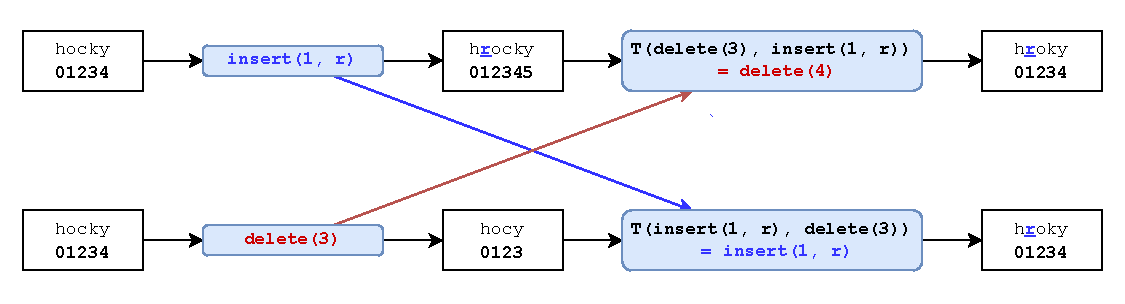
\includegraphics[scale=0.8]{figures/ot-transform}
    \caption[TP1 in action]{TP1 in action. Two sites start from \texttt{hocky}; one inserts \texttt{r} at index~1 while the other deletes index~3. Each site transforms the other's operation against its own, and both arrive at \texttt{hroky}.}
    \label{fig:OTschema}
\end{figure}

TP1 states that applying $\op_1$ and then $\op_2$ transformed against $\op_1$ gives the same document as applying $\op_2$ and then $\op_1$ transformed against $\op_2$ (Figure~\ref{fig:OTschema}). It matters whenever two operations reach two replicas in different orders. An OT algorithm that satisfies TP1 alone is enough to build a client-server system with a single source of truth. In OT systems that do not rely on TP2, convergence requires every operation to be transformed against one shared context~\citep{Xu2016}: for example, the history of operations held on the server can be treated as the authoritative order for every client~\citep{Vidot2000}. When a client receives new operations from the server, it transforms all of its local operations that the server has not yet accepted against them. The server accepts a client's operation only once the client already has every operation the server holds.

TP2 states that transforming a third operation $\op_3$ against $\op_1$ and $\op_2$ gives the same result whichever of the two equivalent orders they were applied in. It is needed only in systems that let two operations be executed on two different document states, that is, where concurrent operations are transformed at different sites rather than against one central history. Algorithms that satisfy TP2 are hard to get right: several published ones were later proven wrong~\citep{OTOverview1}. This difficulty is one reason CRDTs were introduced as an alternative to OT for keeping data consistent and correct across a distributed system.

\section{Conflict-Free Replicated Data Types (CRDTs)}
\label{sec:crdt}

In 2005, \citet{oster2005real} introduced WOOT (WithOut Operational Transformation), the first algorithm that makes the text replicas of a collaborative editor converge without OT. It also preserves the \emph{intention} of an operation, what the operation means to do~\citep{Li2004}. Take the string \texttt{ABCDE}, indexed from $0$, and suppose a client inserts the character \texttt{X} between \texttt{A} and \texttt{B}. The intention is to insert \texttt{X} so that \texttt{A} precedes \texttt{X} and \texttt{X} precedes \texttt{B}. In OT this insertion is written $\texttt{insert}(1, \texttt{X})$; in WOOT it is written $\texttt{insert}(\texttt{A} \prec \texttt{X} \prec \texttt{B})$, where \texttt{A} and \texttt{B} are objects with an identifier unique to each character in the string (Figure~\ref{fig:2:crdt-insert}). WOOT was the starting point for CRDTs, which \citet{Shapiro2011} formally defined in 2011, not only for strings but for many other abstract data types.

\begin{figure}[htbp]
    \centering
    % The same insertion in OT and in a CRDT: ABCDE, a client inserts X between
% A and B. Top: OT addresses characters by index. Bottom: a CRDT addresses
% them by ID, a (client, counter) pair, and keeps a deleted character as a
% tombstone. TikZ libraries: arrows.meta, positioning, fit, backgrounds.
% Colors from thesis.sty.
\begin{tikzpicture}[
  font=\sffamily\footnotesize,
  cell/.style={draw=black!60, line width=0.6pt, fill=white, minimum width=1cm,
    minimum height=0.6cm, inner sep=0pt, font=\ttfamily\small},
  obj/.style={draw=black!60, line width=0.6pt, fill=white, rounded corners=2pt,
    minimum width=0.7cm, minimum height=0.6cm, inner sep=0pt, font=\ttfamily\small},
  new/.style={draw=accent, fill=accentlight, text=accent, font=\ttfamily\small\bfseries},
  tomb/.style={draw=rulegray, fill=codebg, text=rulegray, dash pattern=on 2pt off 1.5pt},
  idx/.style={font=\sffamily\scriptsize, text=black!65, inner sep=1pt},
  oid/.style={font=\ttfamily\scriptsize, text=black!75, inner sep=1pt},
  link/.style={line width=0.6pt, black!60, -{Stealth[length=1.6mm,width=1.3mm]}},
  op/.style={line width=1pt, accent, -{Stealth[length=2.6mm,width=2mm]}},
  oplab/.style={above, font=\ttfamily\footnotesize, text=accent, inner sep=2pt},
  title/.style={font=\sffamily\small\bfseries, text=accent, anchor=west, inner sep=0pt},
  note/.style={font=\sffamily\footnotesize, text=black!70, inner sep=1pt},
  panel/.style={draw=rulegray, line width=0.6pt, rounded corners=3pt, inner sep=0.25cm},
  brace/.style={draw=black!45, line width=0.5pt},
]
  % Character centers: before at x = 0.5 + i, after at x = 8.9 + i.
  % ---- OT: by index ------------------------------------------------------
  \node[title] (t1) at (0,0) {OT: by index};
  \def\yr{-0.85}
  \foreach \ch [count=\i from 0] in {A,B,C,D,E} {
    \node[cell] (o\i) at ({0.5+\i},\yr) {\ch};
    \node[idx] at ({0.5+\i},\yr-0.52) {\i};
  }
  \draw[op] (5.3,\yr) -- node[oplab] {insert(1, X)} (8.1,\yr);
  \foreach \ch [count=\i from 0] in {A,X,B,C,D,E} {
    \ifnum\i=1 \node[cell, new] (p\i) at ({8.9+\i},\yr) {\ch};
    \else \node[cell] (p\i) at ({8.9+\i},\yr) {\ch}; \fi
  }
  \node[idx] at (8.9,\yr-0.52) {0};
  \node[idx, text=accent, font=\sffamily\scriptsize\bfseries] at (9.9,\yr-0.52) {1};
  \foreach \i in {2,...,5}
    \node[idx, text=accent, font=\sffamily\scriptsize\bfseries] at ({8.9+\i},\yr-0.52) {\i};
  % brace under the indices of B..E
  \def\yb{-1.62}
  \draw[brace] (10.5,\yb+0.08) -- (10.5,\yb) -- (14.3,\yb) -- (14.3,\yb+0.08);
  \draw[brace] (12.4,\yb) -- (12.4,\yb-0.08);
  \node[note, below] (n1) at (12.4,\yb-0.08) {B--E shift: each index $+1$};
  \begin{scope}[on background layer]
    \node[panel, fit=(t1)(o0)(p5)(n1)] {};
  \end{scope}

  % ---- CRDT: by identifier ----------------------------------------------
  \node[title] (t2) at (0,-2.75) {CRDT: by identifier};
  \node[note, anchor=west, text=black!60] at (t2.east) {\quad ID = \texttt{(client, counter)}};
  \def\yo{-4.1}
  \foreach \ch/\id [count=\i from 0] in {A/{1,1},B/{1,2},C/{1,3},D/{2,1},E/{2,2}} {
    \node[obj] (q\i) at ({0.5+\i},\yo) {\ch};
    \node[oid] at ({0.5+\i},\yo-0.52) {(\id)};
  }
  \foreach \i [evaluate=\i as \j using int(\i+1)] in {0,...,3}
    \draw[link] (q\i) -- (q\j);
  \draw[op] (5.3,\yo) -- node[oplab] {insert(A $\prec$ X $\prec$ B)} (8.1,\yo);
  % after: A X B C D E, with D deleted (a tombstone)
  \node[obj] (r0) at (8.9,\yo) {A};
  \node[obj, new] (r1) at (9.9,\yo) {X};
  \node[obj] (r2) at (10.9,\yo) {B};
  \node[obj] (r3) at (11.9,\yo) {C};
  \node[obj, tomb] (r4) at (12.9,\yo) {D};
  \node[obj] (r5) at (13.9,\yo) {E};
  \draw[rulegray, line width=0.8pt] ([xshift=-1.5mm]r4.center) -- ([xshift=1.5mm]r4.center);
  \foreach \i [evaluate=\i as \j using int(\i+1)] in {0,...,4}
    \draw[link] (r\i) -- (r\j);
  \node[oid] at (8.9,\yo-0.52) {(1,1)};
  \node[oid, text=accent, font=\ttfamily\scriptsize\bfseries] at (9.9,\yo-0.52) {(3,1)};
  \node[oid] at (10.9,\yo-0.52) {(1,2)};
  \node[oid] at (11.9,\yo-0.52) {(1,3)};
  \node[oid, text=rulegray] at (12.9,\yo-0.52) {(2,1)};
  \node[oid] at (13.9,\yo-0.52) {(2,2)};
  % X remembers its neighbors at insertion time
  \draw[accent, line width=0.6pt, -{Stealth[length=1.6mm,width=1.3mm]}]
    (r1.north) to[out=110, in=70] node[above, font=\sffamily\scriptsize, inner sep=1pt] {left} (r0.north);
  \draw[accent, line width=0.6pt, -{Stealth[length=1.6mm,width=1.3mm]}]
    (r1.north) to[out=70, in=110] node[above, font=\sffamily\scriptsize, inner sep=1pt] {right} (r2.north);
  \node[note, above=1pt of r4, text=black!60, align=center] (n3)
    {D, deleted by another user:\\[-1pt] kept as a tombstone};
  % brace under the IDs of B..E
  \def\yc{-4.87}
  \draw[brace] (10.5,\yc+0.08) -- (10.5,\yc) -- (14.3,\yc) -- (14.3,\yc+0.08);
  \draw[brace] (12.4,\yc) -- (12.4,\yc-0.08);
  \node[note, below] (n2) at (12.4,\yc-0.08) {B--E keep their IDs};
  \begin{scope}[on background layer]
    \node[panel, fit=(t2)(q0)(r5)(n2)(n3)] {};
  \end{scope}
\end{tikzpicture}%

    \caption[The same insertion in OT and in a CRDT]{The same insertion in OT and in a CRDT. OT addresses characters by index, so a concurrent edit can shift the index and the operation must be transformed. A CRDT gives every character a unique ID and inserts the new character between the IDs of its neighbors; a deleted character stays in the sequence as a tombstone.}
    \label{fig:2:crdt-insert}
\end{figure}

A CRDT is an abstract data type that keeps the replicas of a piece of data in agreement across a network. Being an abstract data type means that its semantics are defined by its values and by its operations, so different implementations can realize each operation differently yet behave the same. A CRDT is stored on every client or peer in the network, so memory- and time-efficient implementations matter. Each replica can be modified without coordinating with the others, and if every replica applies the same operations, in any order, they all reach the same final state~\citep{Shapiro2011, CRDToverview2}.

A simple example is a set. A grow-only set, which only supports \texttt{insert(v)}, is trivially a CRDT, because insertions commute. Supporting \texttt{erase(v)} as well needs a rule for an insertion and an erasure of the same element that happen concurrently, for example letting the insertion win, as an observed-remove set does~\citep{Shapiro2011}. In this study, CRDTs are used for text, so the operations involved are the same as in Section~\ref{subsec:OT}: \texttt{insert(pos, c)} and \texttt{delete(pos)}.

In a CRDT for plain text, every character has its own ID. An insertion carries, along with the new character, the IDs of the characters before and after it, and a logical clock that records the order of insertions, the same idea as in WOOT~\citep{oster2005real}. There are two common ways to handle deletion. The first keeps deleted characters in the document forever and only marks them as deleted, a technique known as a \emph{tombstone}~\citep{molli2006tombstone}. The second assigns IDs that are already ordered by position: a character inserted at a given position gets an ID greater than that of the character before it and smaller than that of the character after it. These IDs must be able to grow, so that there is always room for a new ID between two others, and each carries a further identifier unique to its client, so that no two IDs are ever the same. Because the order is in the IDs themselves, a deleted character does not need to be kept.

Compared with OT, which needs only its transformation functions and can represent the document as a plain array of characters, a CRDT needs an additional data structure for every character in the document. Each character gets an ID and becomes an object, linked, implicitly or explicitly, to the characters before and after it, as in the two approaches above.

\section{A Closer Comparison of CRDT and OT}
\label{sec:perbandingan}

Real-time collaborative text editors in industry are still dominated by operational transformation, even though CRDTs are claimed to have better complexity and efficiency~\citep{Sun2019third}. The line between the two is not sharp: at heart, both transform operations so that they commute, and they differ in the parameters they use. A CRDT converts an operation into a representation based on IDs, or other identifiers, and back into a position once it is applied; OT expresses an operation directly by the position of its characters.

OT centers on transformation algorithms that manage the concurrent operations of every client. CRDTs center on the content: the ordering of objects, identifier-based operations, and other representations of edits~\citep{Sun2019Second, Sun2019First}. Proving a CRDT correct is harder than proving an OT algorithm correct, because of the special treatment of its content state~\citep{Sun2019Second}. Every CRDT needs its own criteria to meet its consistency conditions, depending on how it stores its data, and CRDTs for different abstract data types, such as sets, maps and text, each have their own implementation, algorithm and representation. This variety makes convergence harder to prove for CRDTs than for OT, whose basic conditions were proven by earlier research, so that a new OT algorithm only needs to satisfy them~\citep{OTOverview1, Sun2004, oster2005real}.

The two approaches also differ in complexity. In OT, the cost depends on the number of concurrent operations, and nothing is spent on representing the characters of the text as objects. In a CRDT, the cost grows with the size of the document, and setting up a new peer that joins the network also tends to take more time and memory than in OT.

According to \citet{Sun2019Second}, a state-of-the-art OT system takes $O(c)$ time to apply a remote operation and $O(1)$ to apply a local one, with a memory complexity of $O(c)$ or $O(c \cdot m)$, where $c$ is the number of concurrent operations to be transformed and $m$ is the number of users in the network. In practice $c$ is very small ($c \leq 10$), because operations happen in real time, and $m$ is usually at most $5$.

In the same analysis, define $C$ as the size of the content without tombstones, and $C_t$ as the content over the document's whole lifetime, tombstones included. The time complexity of a CRDT operation ranges from $O(C_{t}^{2})$ and $O(C_{t})$ down to $O(1)$ for tombstone-based CRDTs, and is $O(\log C)$ for solutions without tombstones. Memory can be brought down to $O(C)$, both without tombstones and with tombstones plus garbage collection. For typical documents, $10^3 \leq C \leq 10^6$.

\section{Related Work}
\label{sec:penelitian_terkait}

This study uses the Yjs library, which implements the YATA (Yet Another Transformation Approach) CRDT~\citep{Nicolaescu2016yjs}. YATA represents a document as a linked list of objects and uses tombstones, with a garbage collector that cleans up the content of objects marked as deleted. An insertion adds an object \texttt{o(id, left, right, isDeleted, content)} to the list. The \texttt{id} is a pair of the peer's ID and a logical timestamp, the number of operations that peer has performed so far. The fields \texttt{left} and \texttt{right} hold the \texttt{id}s of the objects to the left and to the right of the insertion at the time it was made. The boolean \texttt{isDeleted} records whether the object has been deleted, so the editor knows whether to show it, and \texttt{content} holds the object's data.

Yjs's main optimization is in \texttt{content}, which can hold a whole run of characters rather than one. When an insertion falls inside the content of an existing object, that object is split in two, so each object also stores the length of its content. A deletion simply marks the object as deleted. \citet{Nicolaescu2016yjs} give further details of the implementation and its compression. To synchronize, Yjs peers summarize what they have seen as a \emph{state vector}: the latest logical timestamp received from each peer in the network.

Yjs gained popularity in the few years before this study, and other sequence CRDTs have also been implemented. In Logoot, each object's position identifier combines a position with the ID of the site that created it and that site's logical clock, and a deletion removes the object directly, without leaving a tombstone~\citep{weiss2009logoot}. LSEQ refines how such position identifiers are allocated~\citep{nedelec2013lseq}. Position-based CRDTs like these can suffer from \emph{interleaving}: when two users concurrently type text at the same place, their characters can end up interleaved with each other, rather than kept as two separate runs~\citep{kleppmann2019interleaving}. YATA orders concurrent insertions that share the same neighbors with a deterministic rule based on the IDs of the clients that made them~\citep{Nicolaescu2016yjs}.

RGA (Replicated Growable Array) is an alternative to YATA~\citep{roh2011replicatedrga}. It orders concurrent insertions with a pair of the peer's ID and a logical timestamp greater than any timestamp the peer has seen. In practice, implementations of these algorithms add many optimizations beyond the formal algorithms in their papers, such as garbage collection, compression of the data sent over the network, and the way objects are laid out in memory, and these affect their performance.

\chapter{Research Methodology}
\label{bab:3}

This chapter describes the methodology followed to develop PeerToCP: the research approach, its stages, and the aspects on which the system is evaluated.

\section{Approach and Stages}
\label{sec:pendekatan}

This study takes an experimental approach. Quantitative and qualitative data are collected for each variant of PeerToCP; all variants implement their business logic behind the same user interface. The independent variables are the network architecture of PeerToCP and the method it uses to resolve conflicts and synchronize data. The dependent variables are defined by the aspects of the system listed in Section~\ref{sec:evaluasi}. Quantitative data come from benchmarking and are analyzed descriptively and inferentially, to compare the performance of the variants. Qualitative data come from an objective description of the system. Figure~\ref{bagan} outlines the stages of the study.

\begin{figure}[htbp]
    \centering
    % Stages of the study (English redraw of assets/skripsi/Metode_Penelitian.pdf).
% Five steps, each a box with a bold title and Input / Method / Output rows.
% TikZ libraries: positioning, arrows.meta, fit, calc.
\begin{tikzpicture}[
  font=\sffamily\footnotesize,
  ttl/.style={draw, line width=0.4pt, font=\sffamily\footnotesize\bfseries, align=center,
    text width=#1, inner sep=0.1cm, outer sep=0pt, minimum height=0.65cm,
    execute at begin node={\hyphenpenalty=10000}},
  row/.style={draw, line width=0.4pt, align=left, text width=#1,
    inner sep=0.1cm, outer sep=0pt,
    execute at begin node={\hyphenpenalty=10000}},
  stepbox/.style={draw, line width=1.2pt, inner sep=0pt},
  link/.style={line width=1.2pt, -{Stealth[length=3mm,width=2.6mm]}},
]
  % ---- 1. Problem Formulation (4.2 cm wide) -----------------------------
  \node[ttl=4.0cm, anchor=north] (t1) at (2.1,-3.6) {1. Problem Formulation};
  \node[row=4.0cm, below=0pt of t1] (i1) {Input: a problem for which an alternative solution is sought};
  \node[row=4.0cm, below=0pt of i1] (m1) {Method: literature review and observation};
  \node[row=4.0cm, below=0pt of m1] (o1) {Output: research questions};
  \node[stepbox, fit=(t1)(o1)] (b1) {};

  % ---- 2. Literature Review (4.6 cm wide) -------------------------------
  \node[ttl=4.4cm, anchor=north] (t2) at (7.3,-0.45) {2. Literature Review};
  \node[row=4.4cm, below=0pt of t2] (i2) {Input: research questions, prior work};
  \node[row=4.4cm, below=0pt of i2] (m2) {Method: compare, contrast, synthesize, summarize, criticize};
  \node[row=4.4cm, below=0pt of m2] (o2) {Output: the theoretical foundation and literature review supporting the study};
  \node[stepbox, fit=(t2)(o2)] (b2) {};

  % ---- 3. System Design and Implementation (5.5 cm wide) ----------------
  \node[ttl=5.3cm, anchor=north] (t3) at (13.15,0) {3. System Design and Implementation};
  \node[row=5.3cm, below=0pt of t3] (i3) {Input: architectures and ideas from prior work, optimization gaps, system evaluation, and system development};
  \node[row=5.3cm, below=0pt of i3] (m3) {Method: developing the application system as program code and an architecture design};
  \node[row=5.3cm, below=0pt of m3] (o3) {Output: application code and the system architecture design};
  \node[stepbox, fit=(t3)(o3)] (b3) {};

  % ---- 4. Evaluation and Analysis (5.5 cm wide) -------------------------
  \node[ttl=5.3cm, anchor=north] (t4) at ([yshift=-1.0cm]b3.south) {4. Evaluation and Analysis of System Performance and Correctness};
  \node[row=5.3cm, below=0pt of t4] (i4) {Input: a working application system, system evaluation indicators};
  \node[row=5.3cm, below=0pt of i4] (m4) {Method: experiments, observation, and quantitative and qualitative analysis};
  \node[row=5.3cm, below=0pt of m4] (o4) {Output: evaluation results measured against the performance indicators};
  \node[stepbox, fit=(t4)(o4)] (b4) {};

  % ---- 5. Drawing Conclusions (4.6 cm wide) -----------------------------
  \node[ttl=4.4cm, anchor=north] (t5) at ($(b4.north -| b2.north)+(0,-0.3)$) {5. Drawing Conclusions};
  \node[row=4.4cm, below=0pt of t5] (i5) {Input: evaluation results and research questions};
  \node[row=4.4cm, below=0pt of i5] (m5) {Method: evaluation analysis};
  \node[row=4.4cm, below=0pt of m5] (o5) {Output: conclusions and opportunities for further research};
  \node[stepbox, fit=(t5)(o5)] (b5) {};

  % ---- flow ---------------------------------------------------------------
  \draw[link] (i1.east) -- ++(0.4,0) |- (t2.west);                % 1 -> 2
  \draw[link] (t2.east) -- (t2.east -| b3.west);                  % 2 -> 3
  \draw[link] ([xshift=0.8cm]b3.south west) -- ++(0,-0.5) -| (b2.south); % 3 -> 2
  \draw[link] (b3.south -| b4.north) -- (b4.north);               % 3 -> 4
  \draw[link] (i4.west) -- (i4.west -| b5.east);                  % 4 -> 5
\end{tikzpicture}%

    \caption{Stages of the study.}
    \label{bagan}
\end{figure}

The research problem was motivated by the potential of WebRTC, a web technology, and of several algorithms for synchronizing data in a distributed network, each with its own advantages and disadvantages. The idea also grew out of a practical need in competitive programming: a simple integrated development environment (IDE) in which code is written collaboratively in real time, and in which a program run on one client in the network can be used by every other client in it. This problem gave rise to the research questions of the study.

With those questions as input, a literature review covered the relevant technologies and prior work, and produced the theoretical foundation of the study. The review compared related studies in terms of performance, implementation complexity, how they work, and the proofs of correctness of particular technologies and algorithms, to establish how far the technology on this topic had advanced. The study then moved on to designing and implementing PeerToCP. Three variants were tested: operational transformation (OT) on a client-server architecture, conflict-free replicated data types (CRDTs) on a client-server architecture, and CRDTs on a peer-to-peer architecture. The finished system was evaluated objectively on aspects that represent its performance and scalability. These aspects, given in Section~\ref{sec:evaluasi}, give a clear basis for comparing one implementation with another.

\section{Evaluation Method and Scenarios}
\label{sec:evaluasi}

Based on observations of other real-time collaborative applications, the evaluation covers five essential aspects of each variant of PeerToCP.

\begin{enumerate}
    \item \textbf{Correctness:} every variant of PeerToCP must be correct, meaning that the data replicas kept in sync end up converged and identical.
    \item \textbf{Lightweight:} the application runs with minimal resources and does not disturb other applications on the same operating system. An application that uses excessive resources to do its job is less likely to be adopted.
    \item \textbf{Responsiveness:} the data replicas on every client are synchronized with a low, usable latency. Every client of a real-time collaborative application should see minimal delay, so that the experience feels real-time.
    \item \textbf{Local-first:} an operation is applied to the local replica as soon as the user makes it, without contacting other clients or servers in the network.
    \item \textbf{Scalability:} this aspect is tied to all the others, since the original motivation for a peer-to-peer architecture is to improve service availability by reducing the load on the server. The application's performance depends on the number of clients or users in a network, so scalability matters for a distributed application~\citep{leibnitz2007peer}.
\end{enumerate}

The quantitative and qualitative data from benchmarking are then analyzed, and the conclusions point out opportunities for optimization and for further research.

\chapter{Design and Implementation}
\label{bab:4}

This chapter describes how PeerToCP is designed and built. It introduces the libraries and frameworks it uses and why they were chosen, the design of the system and how it is used, how each of the three variants keeps its replicas consistent, and finally the test scenarios used to compare them.

\section{Libraries and Frameworks}

PeerToCP builds on several third-party libraries, each chosen for a specific reason. The base of the desktop application is Electron. Figure~\ref{fig:4:components} shows how the components described in this section fit together in one PeerToCP client.

\begin{figure}[htbp]
    \centering
    % The components of one PeerToCP client (an Electron app): the renderer
% process with the editor, the shared state and the shell windows; the main
% process with the compiler and node-pty; and the network provider, one per
% variant. TikZ libraries: arrows.meta. Colors from thesis.sty.
\begin{tikzpicture}[
  font=\sffamily\footnotesize,
  proc/.style={draw=accent, line width=0.8pt, rounded corners=3pt, fill=white},
  frame/.style={draw=rulegray, line width=0.6pt, rounded corners=4pt},
  title/.style={font=\sffamily\small\bfseries, text=accent, anchor=west, inner sep=0pt},
  comp/.style={draw=black!60, line width=0.6pt, rounded corners=2pt, fill=white,
    align=center, inner sep=2pt, minimum height=0.85cm},
  alt/.style={draw=black!60, line width=0.6pt, rounded corners=2pt, fill=white,
    dash pattern=on 3pt off 2pt, align=center, inner sep=2pt},
  both/.style={line width=0.6pt, {Stealth[length=2.2mm,width=1.6mm]}-{Stealth[length=2.2mm,width=1.6mm]}},
  one/.style={line width=0.6pt, -{Stealth[length=2.2mm,width=1.6mm]}},
  lab/.style={font=\sffamily\footnotesize, inner sep=1.5pt},
]
  % ---- the client --------------------------------------------------------
  \draw[frame] (0,0) rectangle (15.8,-5.8);
  \node[title, text=black!70] at (0.2,-0.3) {PeerToCP client (Electron app)};

  % ---- renderer process ----------------------------------------------------
  \draw[proc] (0.2,-0.6) rectangle (9.9,-5.55);
  \node[title] at (0.4,-0.9) {Renderer process (Chromium)};
  \node[comp, text width=2.4cm] (cm) at (1.725,-2.6) {CodeMirror~6\\editor};
  \node[comp, text width=2.4cm] (xt) at (1.725,-3.65) {\texttt{xterm.js}\\shell windows};
  % shared state
  \draw[draw=accent, line width=0.6pt, fill=accentlight, rounded corners=3pt]
    (5.7,-1.2) rectangle (9.7,-5.35);
  \node[title, font=\sffamily\footnotesize\bfseries] at (5.85,-1.45) {Shared state};
  \draw[draw=black!60, line width=0.6pt, fill=white, rounded corners=2pt]
    (5.85,-1.7) rectangle (9.55,-4.25);
  \node[anchor=west, inner sep=0pt] at (6.0,-1.95) {Yjs \texttt{Y.Doc} (CRDT variants)};
  \node[comp, minimum width=3.4cm] (ytext) at (7.7,-2.6) {\texttt{Y.Text}\\the code};
  \node[comp, minimum width=3.4cm] (ymap) at (7.7,-3.65) {\texttt{Y.Map} of \texttt{Y.Array}\\the shells};
  \node[alt, minimum width=3.7cm] (collab) at (7.7,-4.8)
    {or, in the OT variant:\\[-1pt]\texttt{@codemirror/collab}};
  % bindings
  \draw[both] (cm) -- (ytext);
  \node[lab, above] at (4.35,-2.6) {\texttt{y-codemirror.next}};
  \draw[both] (xt) -- (ymap);

  % ---- main process ----------------------------------------------------------
  \draw[proc] (10.9,-0.6) rectangle (15.6,-3.9);
  \node[title] at (11.1,-0.9) {Main process (Node.js)};
  \node[comp, text width=4.2cm, minimum height=0.6cm] (gpp) at (13.25,-1.6)
    {system compiler (\texttt{g++})};
  \node[comp, text width=4.2cm] (pty) at (13.25,-3.0)
    {\texttt{node-pty}\\[-1pt]spawns programs in pseudoterminals};
  \draw[one] (gpp) -- node[lab, right] {executable} (pty);
  \node[comp, text width=4.2cm, minimum height=0.6cm, fill=codebg] (prog) at (13.25,-5.15)
    {compiled program};
  \draw[both] (pty) -- node[lab, right] {spawns; I/O} (prog);
  % renderer <-> main
  \draw[both] (9.9,-2.25) -- node[lab, above] {IPC} (10.9,-2.25);

  % ---- network provider -------------------------------------------------------
  \draw[frame, draw=black!60] (0,-6.4) rectangle (15.8,-8.6);
  \node[title, text=black!70] at (0.2,-6.68) {Network provider (one per variant)};
  \foreach \plib/\pdest/\pvar [count=\i] in {
      y-webrtc/{other peers (WebRTC data channels; WebSocket to the signaling server)}/peer-to-peer CRDT,
      y-websocket/{server (WebSocket)}/client-server CRDT,
      rpc-websockets/{OT server (WebSocket RPC)}/client-server OT} {
    \pgfmathsetmacro{\y}{-7.17-0.5*(\i-1)}
    \node[anchor=west, inner sep=0pt, font=\ttfamily\footnotesize\bfseries, text=accent] at (0.4,\y) {\plib};
    \draw[one] (2.75,\y) -- (3.35,\y);
    \node[anchor=west, inner sep=0pt] at (3.5,\y) {\pdest};
    \node[anchor=east, inner sep=0pt, font=\sffamily\footnotesize\itshape, text=black!60] at (15.6,\y) {\pvar};
  }
  \draw[rulegray, line width=0.4pt] (0.4,-7.42) -- (15.6,-7.42);
  \draw[rulegray, line width=0.4pt] (0.4,-7.92) -- (15.6,-7.92);
  % shared state <-> provider
  \draw[both, accent, line width=1pt] (7.7,-5.35) -- node[lab, right, text=accent] {updates} (7.7,-6.4);
\end{tikzpicture}%

    \caption[The components of a PeerToCP client]{The components of a PeerToCP client. The renderer process holds the editor and the shared state; the main process compiles and runs programs; the network provider, which differs between the variants, connects the client to its peers or to the server.}
    \label{fig:4:components}
\end{figure}

\subsection{Main Framework and Code Editor Component}

Electron is a framework for desktop applications that are built like web applications. Its user interface is rendered by Chromium, from HTML (HyperText Markup Language), CSS (Cascading Style Sheets) and JavaScript, and its back end runs on Node.js~\citep{kredpattanakul2018transforming, miglanielectron}, a JavaScript runtime built on Google's V8 engine~\citep{tilkov2010node}.

Electron applications are cross-platform: they run on Windows, GNU/Linux and macOS. Electron gives access to many operating system functions, such as spawning subprocesses and writing files. Because its front end is written with web technologies, an Electron application is also comparatively easy to port to the web, with its functionality limited to what the web allows. Alternatives include Qt, based on C++, and Tauri, based on Rust. Electron was chosen because widely used libraries for operational transformation, CRDTs, WebSocket and WebRTC already exist in JavaScript and can be used directly from Node.js.

An Electron application has a main process that runs when the application starts~\citep{electron}, and each window it opens is a renderer process. The main PeerToCP window is a code editor. Its renderer process can communicate with the main process at any time, and it opens the shell windows in which compiled programs run. The renderer process renders the front end, much like a web page. The central component of the main window is CodeMirror.

CodeMirror is the code editor component, and the user's main point of interaction with the application. It runs in a web browser and models text with an immutable state and modular change operations. It offers many extensions, good accessibility and support for many programming languages. CodeMirror is also the bridge to Yjs, the CRDT library, which already has a CodeMirror binding.

\subsection{Collaboration Components}

Yjs is a library that implements the YATA (Yet Another Transformation Approach) CRDT~\citep{Nicolaescu2016yjs}. Its core is the shared document, \texttt{Y.Doc}, which holds the CRDT data structures: \texttt{Y.Text} for text, and \texttt{Y.Map} and \texttt{Y.Array}, which PeerToCP combines to store the shells and their history. This study uses all three, each with its own abstraction.

Yjs is not tied to a particular network architecture. This study uses two network providers that connect a \texttt{Y.Doc} to other replicas: y-webrtc, for a full-mesh peer-to-peer network, and y-websocket, for a client-server network. Yjs has many active developers and was still being maintained and developed, which is why it was chosen for this study.

For the operational transformation variant, PeerToCP uses @codemirror/collab, CodeMirror's collaborative editing extension. Its network provider, for the client-server architecture, uses a modified rpc-websockets library that supports broadcasting, messaging a specific client, and asynchronous, non-blocking, promise-based remote procedure calls (RPC).

In the OT variant, to keep the program simple, a shell is stored as an append-only array, following OT principles. The operations on a shell are the users' keystrokes. Keystrokes are passed to the terminal as they are, and the program running in the shell decides how to interpret them. A backspace on the shell's input, for example, is recorded by default as the three characters ``$\texttt{\char`\\ b \char`\\ b}$'' (without the quotes): move the cursor left, write a space and move the cursor left again. To collaborate on a shell, every client sends its keystrokes into one shared input channel, without the separate cursors of the code editor.

\subsection{Shell Component}

A shell that runs programs, and that every client in the network can use, needs a library with access to the operating system, to compile and run code. Compilation converts code in a higher-level, human-readable language into binary code a machine can execute~\citep{aho1985compilers}. Besides editing code together, every user can compile a single-file program, using a compiler installed on their operating system. In Node.js, the library that gives access to it is node-pty.

node-pty is a Node.js library that forks processes attached to pseudoterminals. It streams data to and from a process managed by the operating system, and PeerToCP uses it to run compiled command-line (CLI) programs, which have no graphical user interface. It was chosen because it is widely used and cross-platform. The shell also needs a front end, for which PeerToCP uses xterm.js, a component that displays a terminal on a web page. xterm.js takes input from the browser and displays output, and it can be connected to a process running on the system. It has no dependencies, which is why it was chosen.

\section{System Design}

PeerToCP is a desktop application, which runs directly on the user's computer. This makes offline use easier, since no internet connection is needed to open it. Compiling on a peer also needs access to system calls, which web browser APIs do not provide~\citep{v8, spidermonkey}: browsers are designed this way so that scripts cannot attack the computer's operating system directly. Figure~\ref{fig:4:app} shows the application, and Figure~\ref{fig:activity} outlines how it is used.

\begin{figure}[htbp]
    \centering
    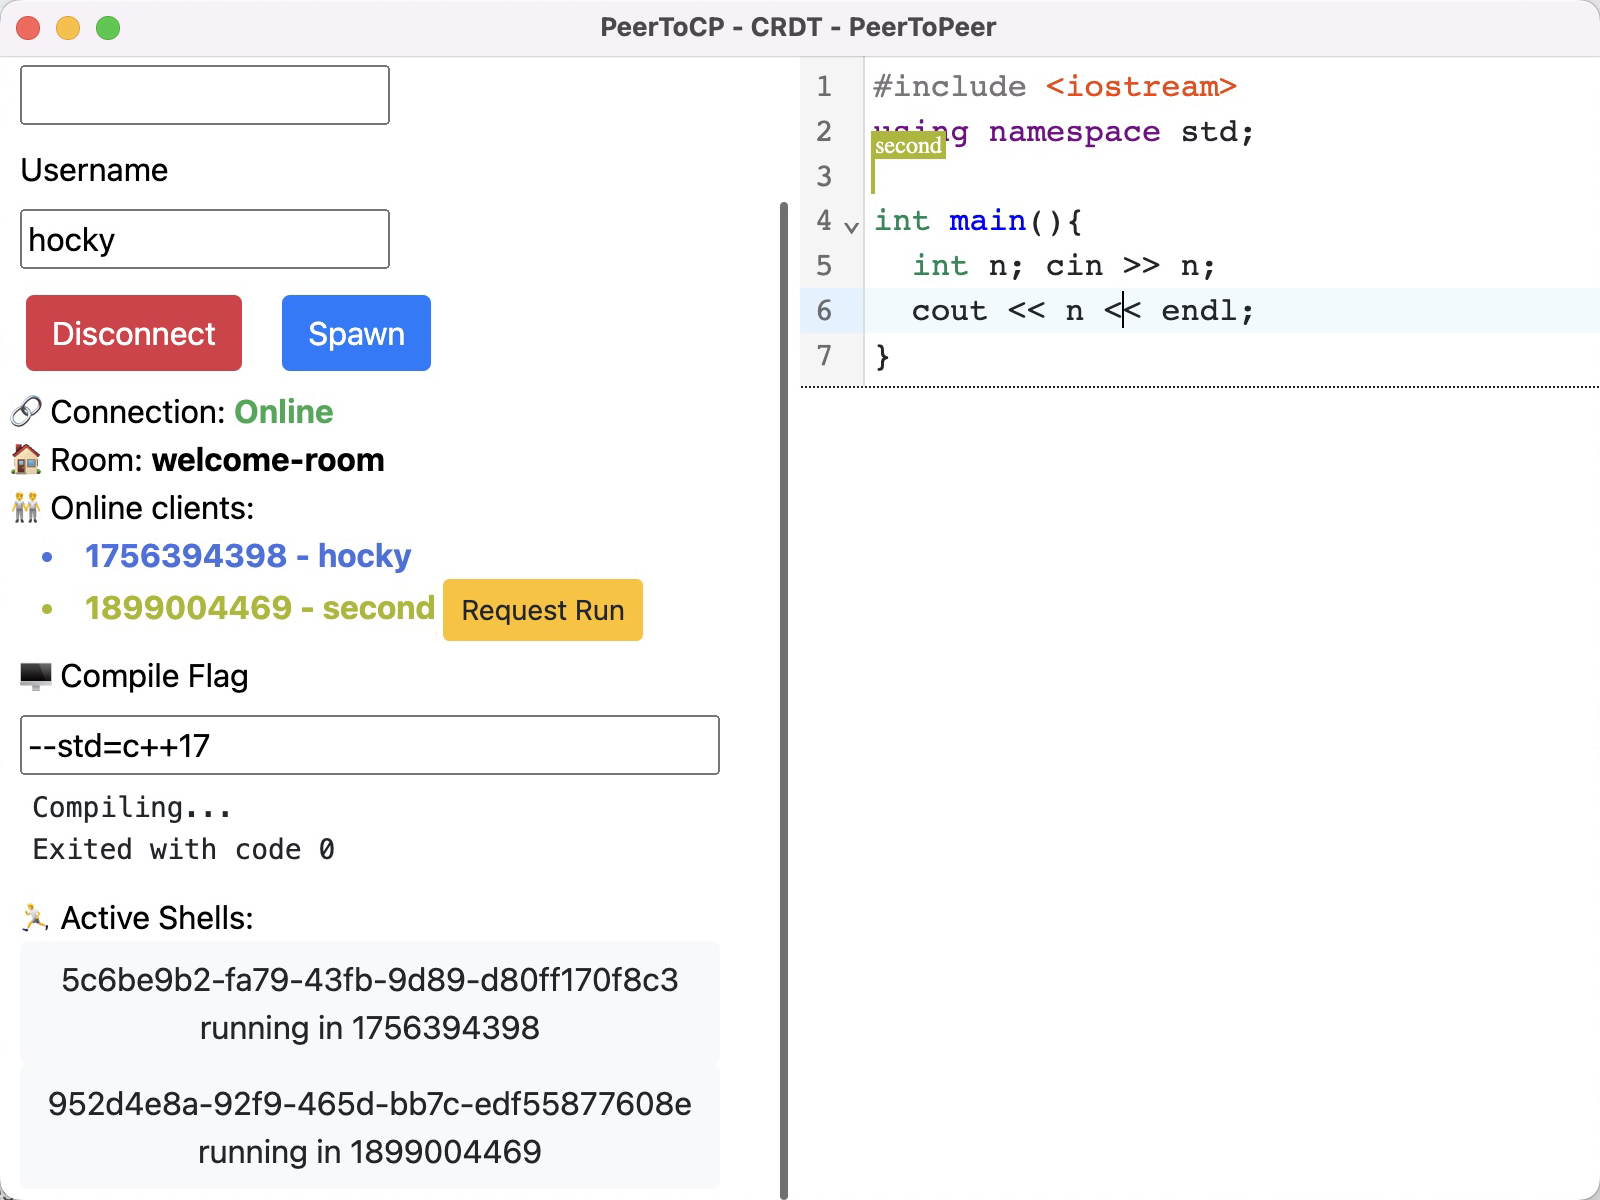
\includegraphics[width=0.82\linewidth]{figures/app-main-window}\\[0.6em]
    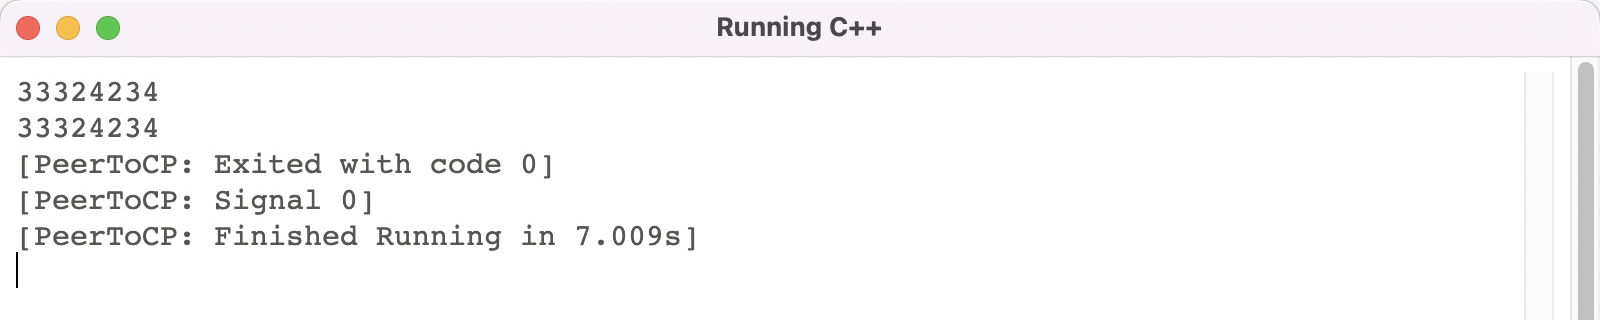
\includegraphics[width=0.82\linewidth]{figures/app-shared-shell}
    \caption[PeerToCP, peer-to-peer CRDT variant]{PeerToCP, peer-to-peer CRDT variant. Top: the main window, with the connection, the room, the online clients (each with a Request Run button), the compiler flags and the list of active shells on the left, and the shared code editor on the right, where another user's cursor, labeled \emph{second}, is visible. Bottom: a shared shell window running a compiled C++ program.}
    \label{fig:4:app}
\end{figure}

\begin{figure}[htbp]
    \centering
    % Activity diagram of the application usage flow (English redraw of
% assets/skripsi/Activity_Diagram.pdf). Three swimlanes: User A, User A's
% System, User B's System. TikZ libraries: arrows.meta, shapes.geometric.
\definecolor{actLaneUserA}{HTML}{DAE8FC}%
\definecolor{actLaneSysA}{HTML}{F8CECC}%
\definecolor{actLaneSysB}{HTML}{FFF2CC}%
\begin{tikzpicture}[
  font=\sffamily\footnotesize,
  >={Stealth[length=2mm,width=1.6mm]},
  flow/.style={->, line width=0.5pt},
  act/.style={draw, rounded corners=3pt, align=center, text width=#1,
    inner sep=2.5pt, minimum height=0.7cm, fill=white,
    execute at begin node={\hyphenpenalty=10000}},
  act/.default=2.3cm,
  dec/.style={draw, diamond, aspect=#1, inner sep=0.5pt, align=center, fill=white},
  merge/.style={draw, diamond, minimum size=0.6cm, inner sep=0pt, fill=white},
  bar/.style={fill=black, inner sep=0pt, minimum height=3.5pt, minimum width=#1},
  guard/.style={fill=white, inner sep=1.5pt},
]
  % ---- swimlanes ---------------------------------------------------------
  \def\laneA{8.9}   \def\laneB{11.9}   \def\laneEnd{15.95}
  \def\headTop{0}   \def\headBot{-0.6} \def\laneBot{-18.25}
  \fill[actLaneUserA] (0,\headTop) rectangle (\laneA,\headBot);
  \fill[actLaneSysA] (\laneA,\headTop) rectangle (\laneB,\headBot);
  \fill[actLaneSysB] (\laneB,\headTop) rectangle (\laneEnd,\headBot);
  \draw (0,\headTop) rectangle (\laneEnd,\laneBot);
  \draw (0,\headBot) -- (\laneEnd,\headBot);
  \draw (\laneA,\headTop) -- (\laneA,\laneBot);
  \draw (\laneB,\headTop) -- (\laneB,\laneBot);
  \begin{scope}[every node/.style={font=\sffamily\footnotesize\bfseries, inner sep=0pt,
      text height=1.6ex, text depth=0.4ex}]
    \node at ({\laneA/2},-0.3) {User A};
    \node at ({(\laneA+\laneB)/2},-0.3) {User A's System};
    \node at ({(\laneB+\laneEnd)/2},-0.3) {User B's System};
  \end{scope}

  % ---- User A ------------------------------------------------------------
  \node[circle, fill=black, minimum size=0.42cm, inner sep=0pt] (start) at (1.6,-1.05) {};
  \node[act=1.9cm] (open) at (1.6,-2.0) {Open the application};
  \node[act] (room) at (1.6,-3.75) {Join a room (the default room when the app first opens)};
  \node[dec=1.6] (conn) at (5.0,-3.75) {Connected to\\the server?};
  \node[act=2.4cm] (access) at (4.4,-6.15) {Access the code document and view the list of program shells};
  \node[act=1.9cm] (edit) at (1.6,-6.95) {Edit the document};
  \node[merge] (d2) at (4.4,-8.0) {};
  \node[act=2.1cm] (send) at (7.3,-8.0) {Send a compilation request with the Request Run button};
  \node[act] (switch) at (1.6,-9.75) {Switch rooms or change display name};
  \node[act=1.9cm] (close) at (7.3,-9.85) {Close the application};
  \node[circle, draw, line width=0.6pt, minimum size=0.5cm, inner sep=0pt] (end) at (7.3,-11.05) {};
  \fill (end) circle (0.15cm);
  \node[act=2.4cm] (openshell) at (4.4,-11.05) {Open one of the program shells};
  \node[merge] (d3) at (4.4,-12.45) {};
  \node[act=2.1cm] (closeshell) at (7.3,-12.45) {Close the shell};
  \node[act=1.9cm] (input) at (4.4,-14.05) {Type input into the shell};
  \node[act=2.1cm] (receive) at (7.3,-14.05) {Receive the compilation result message};

  % ---- User A's System ---------------------------------------------------
  \node[act=2.1cm] (sync) at (10.4,-3.75) {Synchronize program shells and documents};

  % ---- User B's System ---------------------------------------------------
  \node[act=1.6cm] (compile) at (13.6,-8.0) {Compile};
  \node[bar=2.7cm] (fork) at (13.4,-8.85) {};
  \node[dec=1.25] (ok) at (13.6,-10.5) {Compilation\\succeeded?};
  \node[act=2.5cm] (run) at (13.6,-12.45) {Run the program};
  \node[act=2.4cm] (add) at (13.6,-13.75) {Add to the list of running program shells};
  \node[merge] (d5) at (13.6,-15.0) {};
  \node[bar=2.7cm] (join) at (13.4,-15.7) {};
  \node[act=2.8cm] (process) at (13.6,-17.15) {Process keystroke input from any client in the program shell};

  % ---- edges -------------------------------------------------------------
  \draw[flow] (start) -- (open);
  \draw[flow] (open) -- (room);
  \draw[flow] (room) -- (conn);
  \draw[flow] (conn) -- node[guard, above] {Yes} (sync);
  \draw[flow] (conn.south) -- node[guard, right] {No} (conn.south |- access.north);
  \draw[flow] (sync.south) |- ([yshift=0.3cm]access.east);
  \draw[flow] (access) -- (d2);
  \draw[flow] (d2.west) -| (edit.south);
  \draw[flow] (edit.north) |- (conn.south west |- 0,-5.0) -- (conn.south west);
  \draw[flow] (d2) -- (send);
  \draw[flow] (d2.south west) -- (switch.north east);
  \draw[flow] (switch.west) -- (0.18,-9.75) |- (0.9,-4.85) -- (0.9,-4.85 |- room.south);
  \draw[flow] (d2.south east) -- (close.north west);
  \draw[flow] (close) -- (end);
  \draw[flow] (d2) -- (openshell);
  \draw[flow] (openshell) -- (d3);
  \draw[flow] (d3) -- (closeshell);
  \draw[flow] (closeshell.east) -| (8.7,-6.45) -- ([yshift=-0.3cm]access.east);
  \draw[flow] (d3) -- (input);
  \draw[flow] (input.south) |- (process.west);
  % The Request Run line jumps over the close-shell line.
  \draw[flow] (send.east) -- (8.58,-8.0) arc[start angle=180, end angle=0, radius=0.12] -- (compile.west);
  \draw[flow] (compile) -- (compile |- fork.north);
  \draw[flow] (fork.south -| ok.north) -- (ok.north);
  \draw[flow] (fork.south -| 12.25,0) |- (10.4,-9.25) |- (7.3,-13.1) -- (receive.north);
  \draw[flow] (ok) -- node[guard, right] {Yes} (run);
  \draw[flow] (ok.east) -| (15.15,-15.0) -- (d5.east);
  \node[guard] at (15.15,-11.9) {No};
  \draw[flow] (run) -- (add);
  \draw[flow] (add) -- (d5);
  \draw[flow] (d5) -- (d5 |- join.north);
  \draw[flow] (receive.south) |- (12.3,-15.3) -- (join.north -| 12.3,0);
  \draw[flow] (join.south -| 14.45,0) |- (15.45,-16.0) |- (conn.north east |- 0,-1.3) -- (conn.north east);
  \draw[flow] (process.east) -| (15.75,-1.0) -| (conn.north);
\end{tikzpicture}%

    \caption{How the application is used: a high-level activity diagram.}
    \label{fig:activity}
\end{figure}

When users open the application, they join the default room. They can edit the document, and synchronization runs continuously with the publish-subscribe pattern, so updates from other users arrive without having to be checked for, or polled. A user can compile and run the code on their own machine (the \emph{Spawn} button), or send a compilation request to any other user in the network (\emph{Request Run}). PeerToCP delivers the request to the chosen user without involving the other users in the network. The recipient's system compiles the code, runs the program, and adds a shell running it, with its own ID, to the list of shells that every client in the network can access. This list of shells and their contents is stored as a JavaScript object. Figure~\ref{fig:4:request-run} shows this exchange.

\begin{figure}[htbp]
    \centering
    % Request Run and a shared shell: a sequence diagram with three users, B the
% host that compiles and runs the program. Time flows down.
% TikZ libraries: arrows.meta. Colors from thesis.sty.
\begin{tikzpicture}[
  font=\sffamily\footnotesize,
  head/.style={draw=accent, fill=accentlight, line width=0.6pt, rounded corners=2pt,
    minimum width=2.3cm, minimum height=0.75cm, inner sep=2pt,
    font=\sffamily\small\bfseries, align=center},
  life/.style={draw=rulegray, line width=0.6pt},
  msg/.style={line width=0.6pt, -{Stealth[length=2.2mm,width=1.6mm]}},
  rep/.style={msg, accent},
  lab/.style={above, inner sep=1.5pt},
  act/.style={draw=rulegray, fill=codebg, line width=0.6pt, rounded corners=2pt,
    inner sep=2.5pt, minimum height=0.5cm},
  stepnum/.style={circle, fill=accent, text=white, font=\sffamily\scriptsize\bfseries,
    inner sep=0pt, minimum size=4mm},
]
  % ---- lifelines -------------------------------------------------------
  \def\xA{0}  \def\xB{5.2}  \def\xC{10.4}  \def\xN{-1.8}
  \def\yEnd{-6.6}
  \foreach \x in {\xA,\xB,\xC} \draw[life] (\x,-0.375) -- (\x,\yEnd);
  \node[head] at (\xA,0) {User A};
  \node[head] at (\xB,0) {User B (host)};
  \node[head] at (\xC,0) {User C};

  % ---- 1. A asks B to run the code ----------------------------------------
  \node[stepnum] at (\xN,-1.0) {1};
  \node[act] at (\xA,-1.0) {\emph{Request Run} for B};
  \draw[msg] (\xA,-1.65) -- node[lab] {run request (code, flags)} (\xB,-1.65);

  % ---- 2. B compiles --------------------------------------------------------
  \node[stepnum] at (\xN,-2.3) {2};
  \node[act] at (\xB,-2.3) {compile with \texttt{g++}};

  % ---- 3. B runs it in a new shell -------------------------------------------
  \node[stepnum] at (\xN,-2.95) {3};
  \node[act] at (\xB,-2.95) {spawn shell (\texttt{node-pty})};

  % ---- 4. the new shell is shared ------------------------------------------
  \node[stepnum] at (\xN,-3.6) {4};
  \node[act] at (\xB,-3.6) {add the shell to the shell list};
  \draw[rep] (\xB,-4.25) -- node[lab] {shell list update} (\xA,-4.25);
  \draw[rep] (\xB,-4.25) -- node[lab] {shell list update} (\xC,-4.25);
  \fill[accent] (\xB,-4.25) circle (1.4pt);

  % ---- 5. C types into the shell -------------------------------------------
  \node[stepnum] at (\xN,-4.9) {5};
  \draw[msg] (\xC,-4.9) -- node[lab] {keystroke} (\xB,-4.9);

  % ---- 6. the program's output is replicated --------------------------------
  \node[stepnum] at (\xN,-5.55) {6};
  \node[act] at (\xB,-5.55) {append the output to the shell's array};
  \draw[rep] (\xB,-6.2) -- node[lab] {shell output} (\xA,-6.2);
  \draw[rep] (\xB,-6.2) -- node[lab] {shell output} (\xC,-6.2);
  \fill[accent] (\xB,-6.2) circle (1.4pt);

  % ---- note ------------------------------------------------------------------
  \node[draw=rulegray, fill=codebg, line width=0.6pt, rounded corners=2pt, inner sep=3pt,
    font=\sffamily\footnotesize\itshape, text=black!70] at (\xB,-7.1)
    {peer-to-peer: messages go directly between peers; client-server: via the server};
\end{tikzpicture}%

    \caption[Running a program on another user's machine]{Running a program on another user's machine. User A asks user B to run the code; B compiles it, runs it in a new shell and shares that shell with everyone. Keystrokes from any user go to B, the host, and the program's output is replicated to all users. In the peer-to-peer variant the messages travel directly between peers; in the client-server variants they go through the server.}
    \label{fig:4:request-run}
\end{figure}

In Figure~\ref{fig:activity}, how the program shells and the document are synchronized depends on the variant. In the client-server architecture, user A's application connects to and synchronizes with the server; in the peer-to-peer architecture, it connects to and synchronizes with the other peers directly. Likewise, compilation requests and the messages carrying compilation results go directly between peers in the peer-to-peer architecture, but must go through the server in the client-server architecture.

\section{Peer-to-Peer and Client-Server CRDT Variants}
\label{sec:desain_crdt}

Both CRDT variants use the Yjs library. Every peer or client holds a replica, a \texttt{Y.Doc}, which can contain several nested CRDTs. The code is a \texttt{Y.Text}, and the shells are a \texttt{Y.Map} that maps the ID of each shell to a \texttt{Y.Array} holding its contents. The peer-to-peer variant uses the y-webrtc network provider, modified with an interface for sending a message to a specific peer over an RTCDataChannel (Figure~\ref{crdt-p2p}). A keystroke typed by any peer is sent directly to the host peer running the program, which appends the program's response to the array of that shell.

\begin{figure}[htbp]
    \centering
    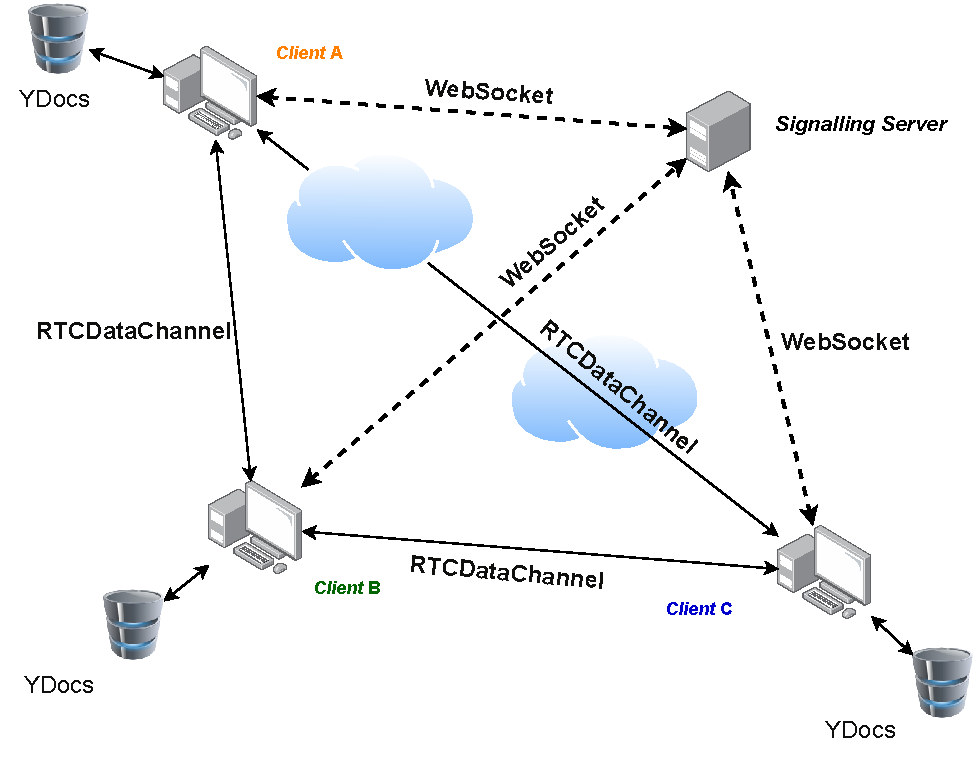
\includegraphics[scale=0.62]{figures/arch-crdt-p2p}
    \caption[The peer-to-peer CRDT variant]{The peer-to-peer CRDT variant: every client keeps a Yjs replica and is connected to every other client over WebRTC data channels; a WebSocket signaling server only introduces the peers to each other.}
    \label{crdt-p2p}
\end{figure}

\begin{figure}[htbp]
    \centering
    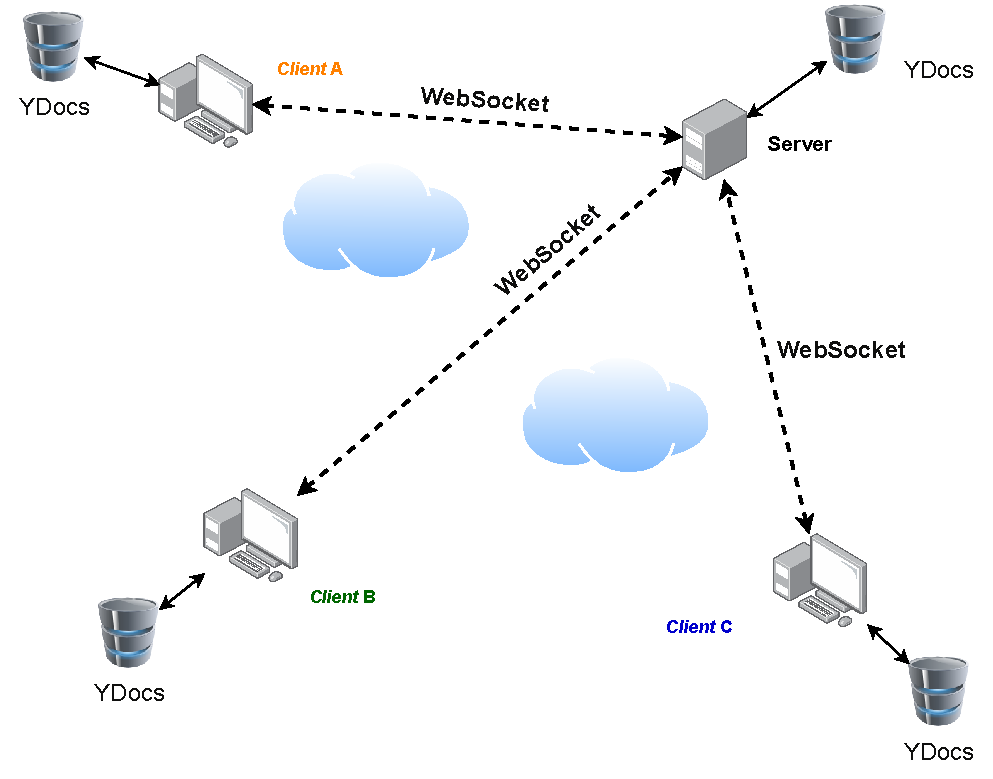
\includegraphics[scale=0.62]{figures/arch-crdt-cs}
    \caption[The client-server CRDT variant]{The client-server CRDT variant: every client keeps a Yjs replica and synchronizes it over WebSocket with the server, which keeps a replica of its own.}
    \label{crdt-cs}
\end{figure}

The two CRDT variants differ only in their network provider. The client-server variant (Figure~\ref{crdt-cs}) uses y-websocket, also modified so that it can send a message to a specific client through the server. A network provider gives every peer or client in a distributed network an abstraction for communicating with the others. In the client-server architecture, the server adds one feature: persistence. The server keeps its own replica of the document, so the document survives even when no client is connected. Besides CRDTs, the client-server architecture is also used with operational transformation, in the third variant compared in this study, whose OT satisfies only TP1.

\section{Client-Server Operational Transformation Variant}
\label{sec:design_ot}

For a document that holds only plain text, operational transformation that satisfies only TP1 can be implemented simply on a client-server architecture. This variant uses the @codemirror/collab library, which implements operational transformation and represents CodeMirror changes as deltas. The client keeps an array of local changes the server does not yet know about. It sends these changes periodically, together with the latest server version it has applied, through RPC over WebSocket; the RPC call does not block the client while it waits for the reply, before the next attempt to send. If the server already has a newer version than the one the changes are based on, it rejects them and tells the client to rebase: to apply the server's newer updates first, before trying again.

\begin{figure}[htbp]
    \centering
    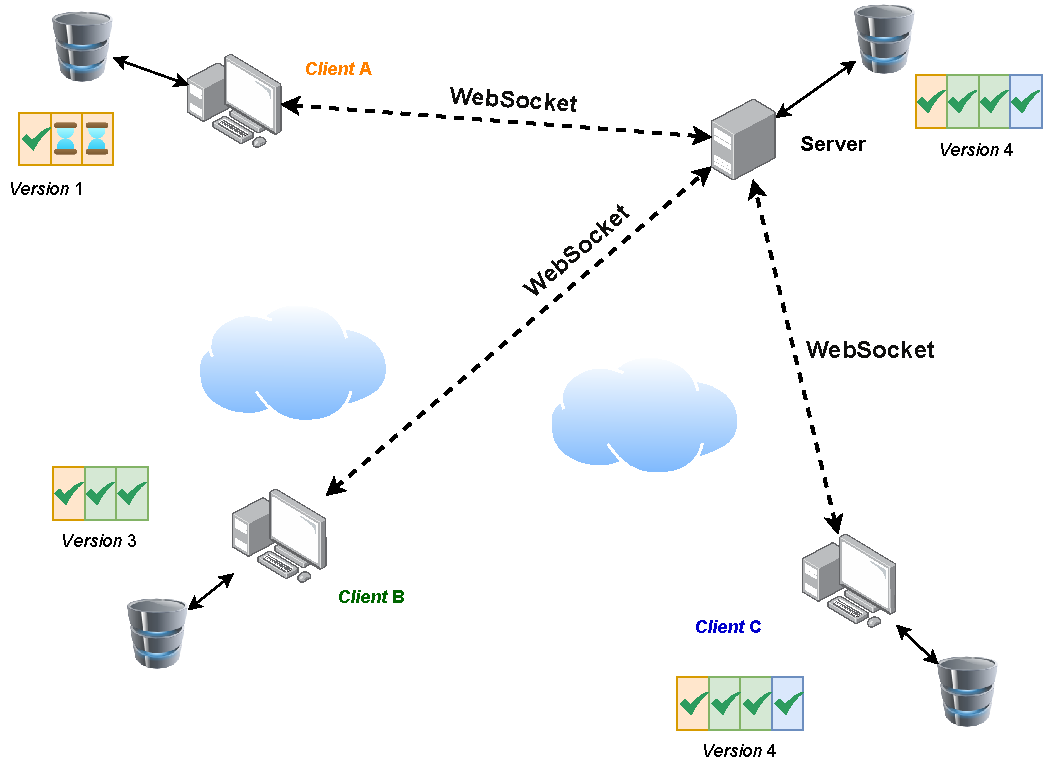
\includegraphics[width=11cm]{figures/arch-ot-cs}
    \caption[The client-server OT variant]{The client-server OT variant: the server holds the authoritative sequence of versions, and each client keeps its pending local changes until the server accepts them.}
    \label{fig:websocket_ot}
\end{figure}

Remote changes received from the server are transformed against the local changes the server does not know about yet; the local changes are then replaced by their versions transformed against the remote ones, and these are what the client sends next. Operational transformation happens only on the clients, and the server applies changes strictly in order, so every replica of the document converges to the same text. Figure~\ref{fig:websocket_ot} shows this architecture.

\begin{figure}[htbp]
    \centering
    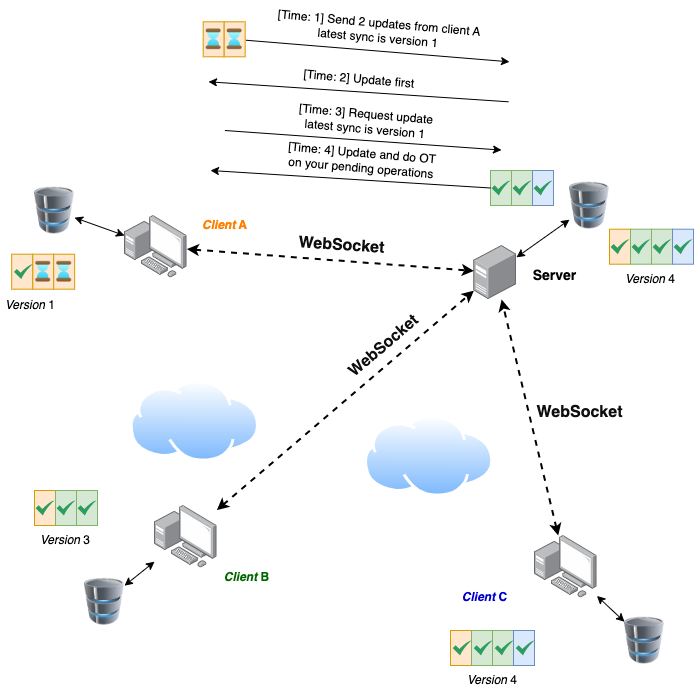
\includegraphics[width=7cm]{figures/ot-sync-1}\hfill
    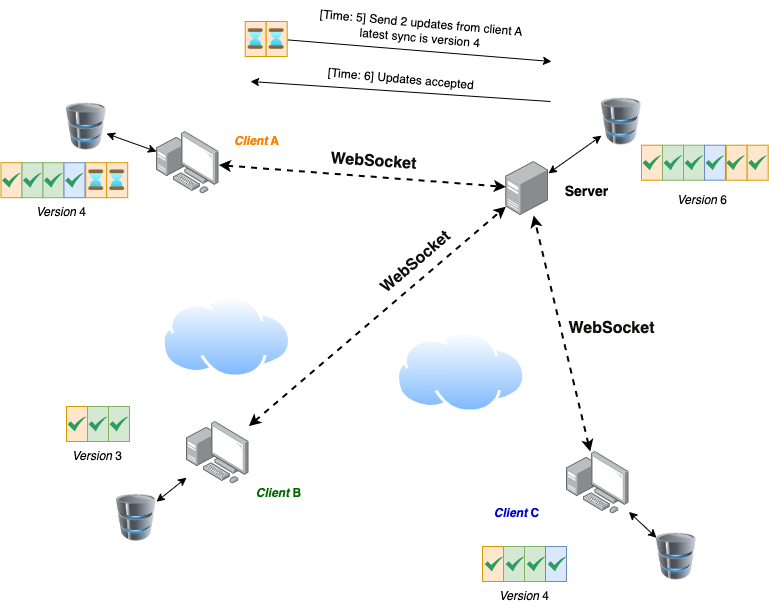
\includegraphics[width=7cm]{figures/ot-sync-2}
    \caption[Synchronization in the OT variant]{Synchronization in the OT variant. Left: client A's two pending updates are rejected, because the server has moved on. Right: after pulling the server's new operations and transforming its own against them, client A's updates are accepted.}
    \label{fig:ots}
\end{figure}

Figure~\ref{fig:ots} shows an example. The server cannot accept client A's two pending updates until client A has all of the server's latest versions. After pulling updates and receiving three new operations from the server, client A transforms its two pending updates against them. Client A's local document is now at version~4, and it can send its updates. The server appends client A's two operations, which brings it to version~6.

The shells of running programs work the same way. When a client types a keystroke into one of the active shells, the keystroke is sent through a similar mechanism, but routed to the client that hosts, that is, runs, the program. The host sends the changes to the shell to the server periodically, as long as there are changes the server has not received, and when a change arrives the server notifies every client to pull it. Because only the host produces the shell's contents, these updates need no transformation function, unlike plain-text OT. Positions need no mapping either, because the cursor is always after the last character. Applying updates serially in this way prevents race conditions during network disruptions.

\section{Evaluation Design}
\label{sec:desain_evaluasi}

The three architectures are back ends for the same editor interface, so the benchmark measures, end to end, what users experience. It consists of scenarios that cover the aspects being tested, run under conditions kept as identical as possible across the variants.

The system is evaluated on the Compute Engine service of Google Cloud Platform. Each variant has its server on an instance in the \texttt{asia-southeast1-b} zone, on an \texttt{e2-medium} machine with 2~vCPUs, 4~GiB of RAM and Debian~11. This machine type was chosen so that the server's specifications do not limit the benchmark. No relay (TURN) server is provided for peers that cannot connect to each other in the peer-to-peer variant: the study assumes that the WebRTC connections between peers can always be set up.

The users are \texttt{e2-small} virtual machines with 2~vCPUs, 2~GiB of RAM and Debian~11, all in the \texttt{asia-southeast2-a} zone, a region close to the servers, to approximate real-world use of PeerToCP. Four test scenarios are run, each with $n \in \{2, 4, 8\}$ users, to show how the system scales with the number of users in a network. The largest value of $n$ reflects the expected maximum number of users of PeerToCP, which is no more than eight. Table~\ref{tab:skenarios} summarizes the scenarios.

\begin{table}[htbp]
\centering
\caption{Test scenarios.}
\label{tab:skenarios}
\begin{tabular}{@{}clccc@{}}
\toprule
\textbf{Scenario} & \textbf{Component} & \textbf{Measures latency} & \textbf{Duration (s)} & \textbf{Disconnection} \\
\midrule
1 & Code editor & No  & 180            & Yes, 30\,s \\
2 & Shell       & No  & $\approx$100   & Yes, 20\,s \\
3 & Code editor & Yes & 120            & No \\
4 & Shell       & Yes & $\approx$100   & No \\
\bottomrule
\end{tabular}
\end{table}

\paragraph{Scenario 1: editing under stress.} The first scenario simulates a stream of edits in the code editor, with each number of peers $n$, for the scalability aspect. Every 100~milliseconds, for three minutes, each client performs one of three random operations, chosen with equal probability:

\begin{enumerate}
    \item inserting (\texttt{insert}) a random string of 2 to 5 characters;
    \item deleting (\texttt{delete}) a range of 1 to 3 characters;
    \item replacing (\texttt{replace}) a range of 2 to 5 characters with a random string of 2 to 5 characters.
\end{enumerate}

On each client, these operations grow the document by about 5 characters per second on average, and change about 41.67 characters per second, insertions and deletions together. The tests start at the same time on every client, using the operating system's clock, which is synchronized by default. Some error between the clocks is unavoidable and is assumed to be negligible; identical instances for every client reduce the bias from differences between them. In addition, each client disconnects from the network for 30~seconds, starting at a random time between 60 and 90~seconds into the test, so that the disconnection always falls between the first and the last minute. At the end, every editor is connected again, for a final synchronization with the other users. While an editor is disconnected, it keeps performing \texttt{insert}, \texttt{delete} and \texttt{replace} operations, which tests the local-first aspect.

The first scenario is a stress test of the editing that can happen in the real world. After the test, the system waits for one minute, to give synchronization time to finish. The time of the last update is recorded and compared, for the responsiveness and scalability aspects. The hash of the final document is recorded on every client and compared across them, for the correctness aspect. The RAM, CPU and network activity of the first two clients of each run, and of the server, are recorded with the Netdata monitoring agent, for the lightweight and scalability aspects.

\paragraph{Scenario 2: a shared shell under disconnection.} The second scenario uses the same environment as the first. It tests the shell with each number of clients $n$, by running a C++ program that prints 100 random unsigned 64-bit integers, waiting a random 500 to 1500~milliseconds before each one. Meanwhile, a 20-second network disconnection starts at a random time 10 to 40~seconds after the program starts. As in the first scenario, the last synchronization time, the device activity and the hash of every shell on every client are recorded and compared, to make sure that every user ends up with the same shell replica.

\paragraph{Scenarios 3 and 4: latency.} The last two scenarios measure the latency of the code editor and of the shell, respectively. In the third scenario, the $n$ peers are set up as before, and each performs two kinds of operation: inserting a timestamp into the editor, and replacing a range of 10 to 15 characters with a timestamp. Each operation waits a random 500 to 1000~milliseconds, so that the operations do not all happen at a fixed period. Every client captures the timestamps it receives and measures the latency as the time between a timestamp being written and its arrival at another client. In the fourth scenario, every client runs a C++ program that prints 100 timestamps, with a random delay of 500 to 1500~milliseconds between them. Every client captures each timestamp and measures its latency in the same way, as the time between the host of the shell (the user running the program) adding the timestamp and each other user receiving it. Scenarios 3 and 4 have no disconnections, so that the data for the responsiveness aspect are as accurate as possible.

\chapter{Results and Discussion}
\label{bab:5}

This chapter presents and analyzes the results of the evaluation, run according to the scenarios of Section~\ref{sec:desain_evaluasi}. The analysis is organized by the aspects defined in Chapter~\ref{bab:3}, to give a clear picture of how each variant performs and what resources it needs to do so. Along the way, it considers which variant of PeerToCP is preferable and why, and points out weaknesses of the system as directions for future development.

\section{The Local-First and Correctness Aspects}
\label{sec:5:correctness}

These two aspects go together. In Scenarios 1 and 2, the local-first aspect was tested by disconnecting clients at random while every user kept changing their local data offline. The changes were indeed local-first: they could still be made, and were applied immediately, while the client was offline, and when the client rejoined the network its data was brought up to date with the changes made in the meantime.

In the experiments, the clients of every variant ended each scenario with the same document hash, that is, in the same final state. The exception is Scenario 1 with eight clients, in which some clients of the client-server OT variant could not reconnect after their disconnection. The likely cause is the inefficient way this variant transmits data, which pushed the bandwidth it needed beyond the limits of the test environment.

Scenario 1 with eight clients was run up to three times for the OT variant, and in each run one or two clients could not reconnect. As described in Section~\ref{sec:desain_evaluasi}, every client was disconnected at a random time, for the same duration. Figure~\ref{fig:2-23} shows the incoming network data of the first and second clients of each variant in this scenario.

\begin{figure}[htbp]
 \centering
 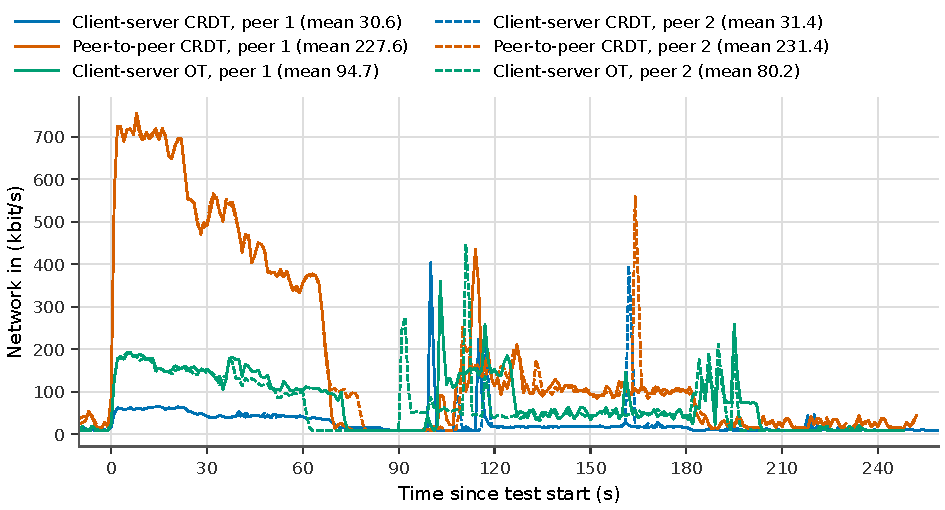
\includegraphics[width=\linewidth]{figures/s1-n8-peers-network-in}
 \caption{Incoming network data of the first and second clients, Scenario 1, $n = 8$.}
 \label{fig:2-23}
\end{figure}

The incoming traffic in Figure~\ref{fig:2-23} looks normal: the updates received are not very large. Figure~\ref{fig:2-25}, however, shows that the first client of the OT variant, which was disconnected at second 72 and reconnected at second 102, then sent a large amount of data for about 20 seconds. The same holds for the second client, disconnected at around second 60 and reconnected at second 90: right after a client reconnects, its outgoing traffic spikes. With many users in one document, disconnections and reconnections at similar times can make this variant unreliable.

\begin{figure}[htbp]
 \centering
 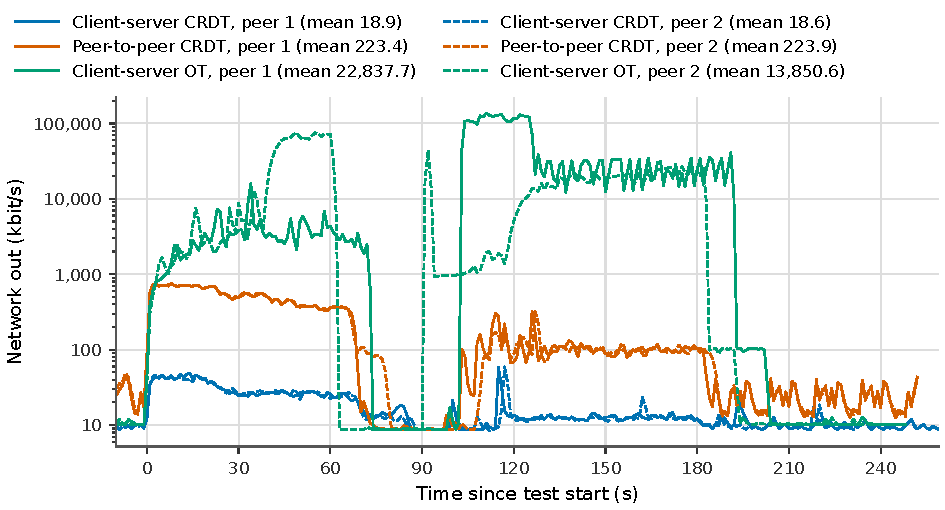
\includegraphics[width=\linewidth]{figures/s1-n8-peers-network-out}
 \caption[Outgoing network data of the first and second clients, Scenario 1, $n = 8$, on a logarithmic scale]{Outgoing network data of the first and second clients, Scenario 1, $n = 8$, on a logarithmic scale. The OT clients send up to a thousand times more than the CRDT clients, in bursts after their reconnection.}
 \label{fig:2-25}
\end{figure}

An update sent right after the connection is restored tends to be large, because it gathers the operations made while the client was offline. When it is sent, the server is also receiving updates from many other clients. The OT algorithm implemented here accepts an update only if the client's latest version matches the server's; otherwise, the server rejects the update and asks the client to pull first. Meanwhile, the backlog of large updates keeps being resent, and can saturate the server's bandwidth.

\begin{figure}[htbp]
 \centering
 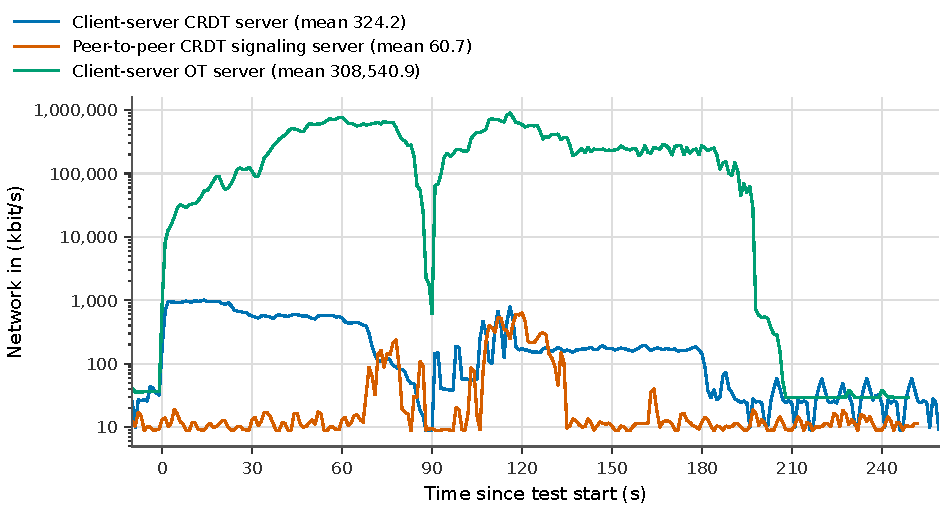
\includegraphics[width=\linewidth]{figures/s1-n8-server-network-in}
 \caption[Incoming network data of the servers, Scenario 1, $n = 8$, on a logarithmic scale]{Incoming network data of the servers, Scenario 1, $n = 8$, on a logarithmic scale. The signaling server of the peer-to-peer variant stays close to zero.}
 \label{fig:2-24}
\end{figure}

The traffic into the server of the client-server OT variant can exceed 800{,}000 kilobits per second, that is, 100 megabytes per second. Figure~\ref{fig:2-24} shows that its mean rate is about 950 times that of the client-server CRDT variant. The signaling server of the peer-to-peer CRDT variant, by contrast, shows almost no activity: it does not take part in the data exchange, because the peers communicate directly.

In Scenario 1, the CRDT variants are more reliable, because updates to the document can be merged in any order. Other likely factors are the implementation of the WebSocket provider and the compression and encoding Yjs uses. In the OT variant, updates also pile up because of large change operations, which take longer to arrive than the smaller updates of other clients. As a result, some clients have to pull repeatedly before they can push their own update, whenever their local version differs from the server's. This in turn affects two other aspects: scalability and responsiveness.

\section{The Scalability and Responsiveness Aspects}
\label{sec:5:latency}

The latency of the code editor was measured in Scenario 3, which, unlike Scenarios 1 and 2, has no disconnections. Each user measured the delay with which data from every other user arrived, recorded when the document data arrived, and these latencies were averaged over the $n$ users in the network. Table~\ref{tab:latency-3} gives the latency of nonlocal operations, that is, operations made by the other users in the network. The peer-to-peer CRDT variant has the lowest latency, although the gap between it and the client-server CRDT variant narrows as $n$ grows. The latency of the client-server OT variant is more than twice that of the client-server CRDT variant, nearly four times at $n = 8$, with spikes of about two seconds at $n = 8$.

\begin{table}[htbp]
 \centering
 \caption{Latency of nonlocal operations in Scenario 3 (shared code editor), in milliseconds.}
 \label{tab:latency-3}
 \begin{tabular}{@{}c rrr rrr rrr@{}}
 \toprule
 & \multicolumn{3}{c}{\textbf{Peer-to-peer CRDT}} & \multicolumn{3}{c}{\textbf{Client-server CRDT}} & \multicolumn{3}{c}{\textbf{Client-server OT}} \\
 \cmidrule(lr){2-4}\cmidrule(lr){5-7}\cmidrule(l){8-10}
 $n$ & Mean & Median & Max & Mean & Median & Max & Mean & Median & Max \\
 \midrule
 2 & 23.30 & 21 & 76  & 39.50 & 38 & 134 & 87.42  & 84  & 168 \\
 4 & 34.00 & 30 & 223 & 46.10 & 42 & 220 & 98.84  & 86  & 1{,}225 \\
 8 & 55.56 & 47 & 313 & 63.84 & 56 & 308 & 235.62 & 151 & 2{,}010 \\
 \bottomrule
 \end{tabular}
\end{table}

As for scalability: when all users are close to one another (in this experiment, all peers were in the same zone, in Indonesia), the peer-to-peer architecture performs better than the client-server one for the values of $n$ tested. The narrowing gap in Table~\ref{tab:latency-3} suggests, however, that the client-server CRDT variant may offer better responsiveness for larger $n$, or when the peers are farther apart.

Figure~\ref{fig:5:summary-latency} summarizes the latency measurements of Scenarios 3 and 4 against the number of users.

\begin{figure}[htbp]
 \centering
 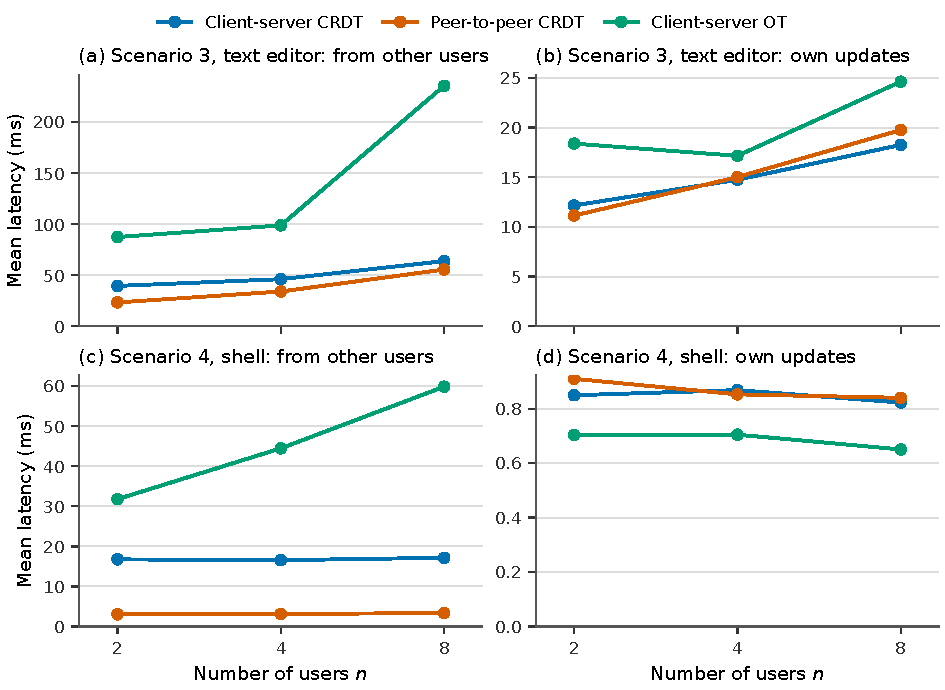
\includegraphics[width=\linewidth]{figures/summary-latency}
 \caption[Mean latency against the number of users $n$]{Mean latency against the number of users $n$. (a) and (c): updates from other users, as in Tables~\ref{tab:latency-3} and~\ref{tab:latency-4}; (b) and (d): the time to apply a user's own updates.}
 \label{fig:5:summary-latency}
\end{figure}

Part of the difference in latency may also come from the algorithm that keeps the replicas identical. To isolate it, the time to apply local changes was measured for each variant. A local operation here is one that a user makes on their own document: it is local-first and involves no network transmission. Figure~\ref{fig:12-5} shows only a small difference between the variants, about 5~ms on average, and small spikes, which can occur when characters are inserted or deleted at particular random positions. Note that the costs of CRDT and OT scale differently: the time complexity of OT depends on the number of concurrent operations, while that of a CRDT depends on the number of characters, that is, on the size of the document.

\begin{figure}[htbp]
 \centering
 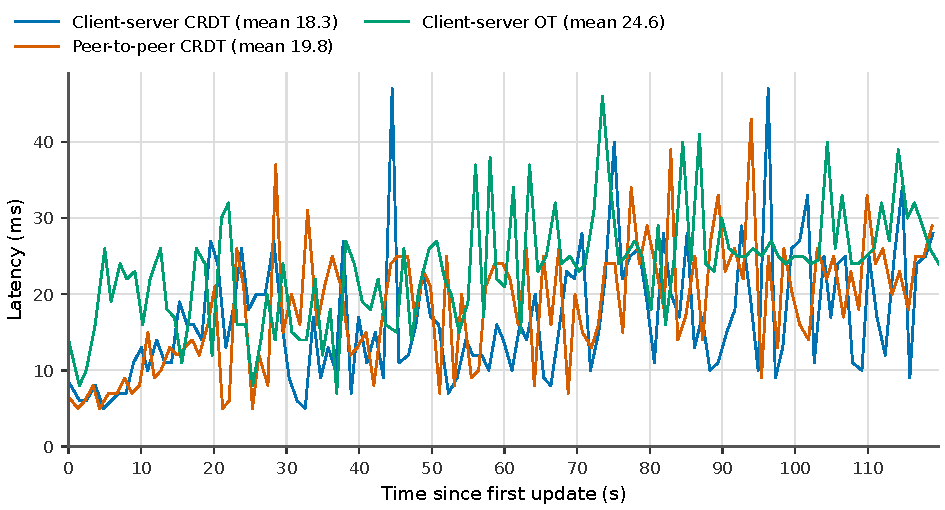
\includegraphics[width=\linewidth]{figures/s3-n8-latency-self}
 \caption{Time to apply local operations in the code editor, Scenario 3, $n = 8$.}
 \label{fig:12-5}
\end{figure}

The total latency is the time to apply local and nonlocal operations plus the network transmission time, which differs between the architectures. Figure~\ref{fig:7-5} shows larger differences between the variants, and several latency spikes over the course of Scenario 3. They have two likely causes: the time to resolve nonlocal operations, and the pile-up of updates illustrated in Figure~\ref{diagram:snowball}.

\begin{figure}[htbp]
 \centering
 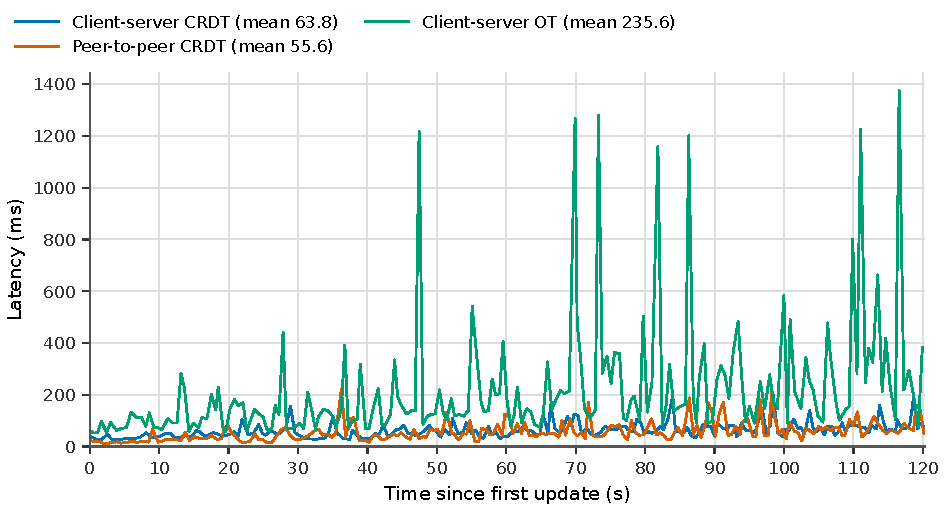
\includegraphics[width=\linewidth]{figures/s3-n8-latency-others}
 \caption{Latency of nonlocal operations in the code editor, Scenario 3, $n = 8$.}
 \label{fig:7-5}
\end{figure}

\begin{figure}[htbp]
 \centering
 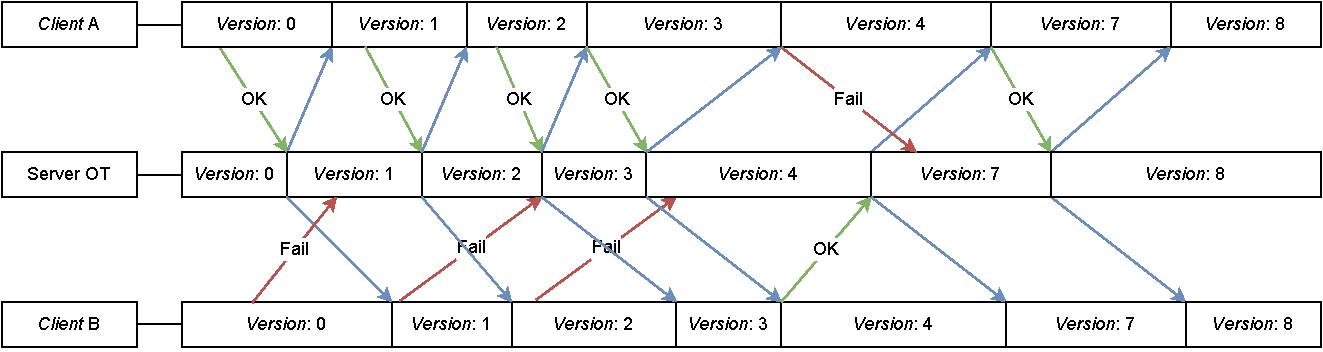
\includegraphics[width=\linewidth]{figures/ot-snowball}
 \caption[Updates piling up in the OT variant]{Updates piling up in the OT variant. Green arrows are pushes the server accepts, red arrows pushes it rejects because the client is behind, and blue arrows pulls. Client B's pushes keep failing while client A keeps getting its own in first.}
 \label{diagram:snowball}
\end{figure}

In the client-server OT architecture, the server does not accept an update from a client that does not have its latest version yet. Updates pile up when a client cannot get its data accepted, because its update keeps growing while other clients always get theirs in first. This holds back the updates of one or more clients, and makes the data the clients send, and the server receives, much larger than in the other variants.

In realistic use, this should not happen often, because users do not insert, delete and change characters as fast and as simultaneously as in Scenario 1. Repeated copy-and-paste operations could cause it, since they change many characters at once. Such operations, however, usually come with enough time between them for every client to update its replica before the next large change.

Scenario 4 tests the latency of the shared shell, which every user in the network can use at the same time; Table~\ref{tab:latency-4} summarizes it. In the code editor, applying a local operation took about 10 to 25~ms on average (Figure~\ref{fig:12-5}). The shell's data structure is a simple append-only list, so applying an operation takes almost no time in any variant, and the variants show no notable difference (Figure~\ref{fig:13-5}).

\begin{table}[htbp]
 \centering
 \caption{Latency of nonlocal operations in Scenario 4 (shared shell), in milliseconds.}
 \label{tab:latency-4}
 \begin{tabular}{@{}c rrr rrr rrr@{}}
 \toprule
 & \multicolumn{3}{c}{\textbf{Peer-to-peer CRDT}} & \multicolumn{3}{c}{\textbf{Client-server CRDT}} & \multicolumn{3}{c}{\textbf{Client-server OT}} \\
 \cmidrule(lr){2-4}\cmidrule(lr){5-7}\cmidrule(l){8-10}
 $n$ & Mean & Median & Max & Mean & Median & Max & Mean & Median & Max \\
 \midrule
 2 & 3.05 & 3 & 5  & 16.75 & 17 & 19 & 31.79 & 30    & 170 \\
 4 & 3.13 & 3 & 6  & 16.55 & 17 & 21 & 44.47 & 32    & 309 \\
 8 & 3.36 & 3 & 19 & 17.16 & 17 & 35 & 59.86 & 30.33 & 551 \\
 \bottomrule
 \end{tabular}
\end{table}

\begin{figure}[htbp]
 \centering
 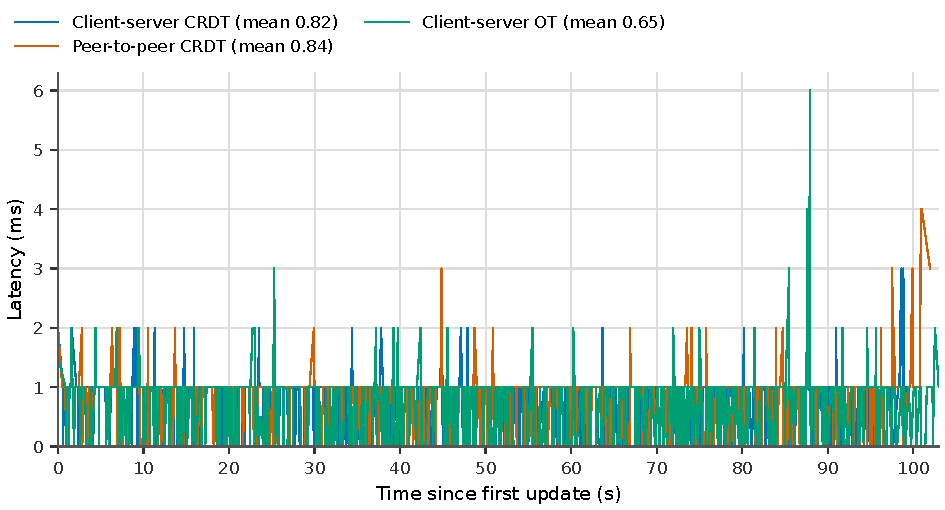
\includegraphics[width=\linewidth]{figures/s4-n8-latency-self}
 \caption{Time to apply local operations in the shared shell, Scenario 4, $n = 8$.}
 \label{fig:13-5}
\end{figure}

This is because appending to an append-only array takes amortized constant time. For the shell, scalability is therefore mainly a matter of how efficiently the data is transmitted, and shell updates in the OT variant suffer from the same problem as in Scenarios 1 and 3, as Figure~\ref{fig:9-5} shows.

Another reason why OT is slower than the client-server CRDT is its communication mechanism. The Yjs CRDT implementation encodes and decodes updates in a compact binary form, which makes transmitting large data faster, and a CRDT does not need updates to be applied in order. The OT variant, in contrast, uses the same update mechanism for the shell as for its code editor.

\begin{figure}[htbp]
 \centering
 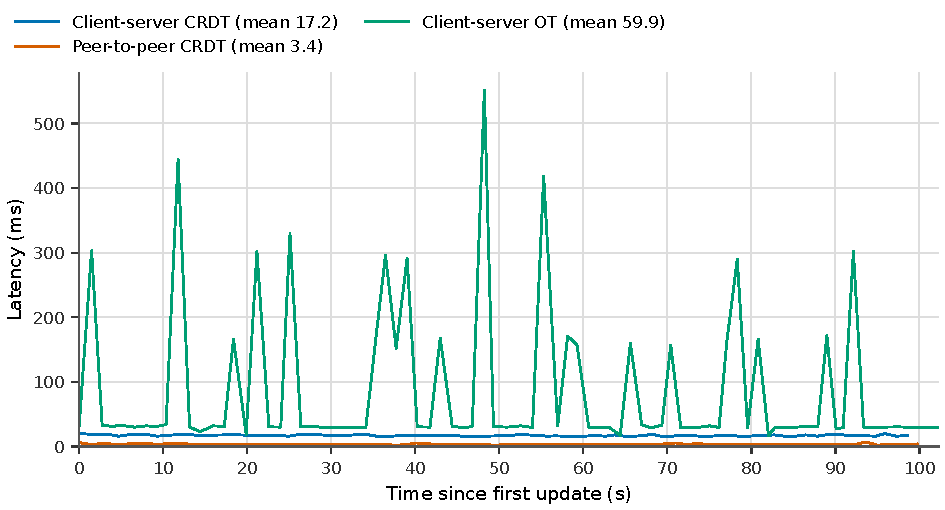
\includegraphics[width=\linewidth]{figures/s4-n8-latency-others}
 \caption{Latency of nonlocal operations in the shared shell, Scenario 4, $n = 8$.}
 \label{fig:9-5}
\end{figure}

In this experiment, the peers of the peer-to-peer variant were close to one another, in the same zone, and their latency was lower than in both client-server variants, whose traffic must pass through the server first. For $n \leq 8$, the peer-to-peer variant gives the best responsiveness of all the variants. For $n > 8$, or for peers farther apart, the client-server CRDT variant is expected to be worth considering as the better alternative.

Peers in the WebRTC-based variant may also be unable to connect to one another at all. A TURN relay server can then forward their traffic, at a latency that further experiments would have to measure. A better OT algorithm is also worth considering: in theory, its constant-time append operations could give the shell lower latency, by exploiting the append-only array and the fact that only the host of a shell forwards its interaction data. The CRDT data structure for the shell could likewise be modified to exploit these properties.

The system could also choose the best architecture automatically: peer-to-peer without a relay server, as in this experiment; peer-to-peer with a relay server, for peers that cannot connect directly over WebRTC; or client-server, when a network group has many clients. For latency, this choice could rest on a simple metric such as the ping between users, measured in the background. Other factors must be weighed as well, above all the lightweight aspect: how much processing, bandwidth and memory the server and the users must provide.

\section{The Lightweight Aspect}
\label{sec:5:lightweight}

This aspect describes how much computing resources each user and the server need. All RAM measurements were normalized to zero just before each test started, so that their growth can be compared. On the clients, the Electron application runs on Chromium, which has its own garbage collection and caching~\citep{chromium}, so memory is more meaningfully measured relative to its size just before the test. At the start, each server uses relatively little RAM, under 20~MiB, while each client starts at about 200~MiB, because the Electron framework runs a Chromium web browser for its front end.

\begin{table}[htbp]
 \centering
 \caption[Mean resource usage of the client application in Scenario 1]{Mean resource usage of the client application in Scenario 1. CPU in percent of one vCPU, RAM growth in MiB, network rates in kbit/s. Each value is the mean of the first two clients.}
 \label{tab:resource-client-1}
 \begin{tabular}{@{}llrrr@{}}
 \toprule
 \textbf{Variant} & \textbf{Metric} & $n = 2$ & $n = 4$ & $n = 8$ \\
 \midrule
 Peer-to-peer CRDT & CPU     & 39.20     & 60.14     & 62.29 \\
                   & RAM     & 16.58     & 19.24     & 21.30 \\
                   & Net in  & 28.52     & 96.17     & 229.48 \\
                   & Net out & 28.04  & 93.98  & 223.63 \\
 \midrule
 Client-server CRDT & CPU     & 33.96    & 57.39     & 56.89 \\
                    & RAM     & 14.93    & 19.13     & 20.95 \\
                    & Net in  & 19.47    & 27.69     & 30.97 \\
                    & Net out & 19.76 & 21.21  & 18.73 \\
 \midrule
 Client-server OT & CPU     & 47.79       & 73.29       & 65.26 \\
                  & RAM     & 25.95       & 31.17       & 36.34 \\
                  & Net in  & 62.24       & 99.81       & 87.42 \\
                  & Net out & 12{,}962.05 & 28{,}872.47 & 18{,}344.15 \\
 \bottomrule
 \end{tabular}
\end{table}

In Table~\ref{tab:resource-client-1}, 100\% CPU utilization means that the application fully uses one vCPU core. RAM usage and incoming data of the peer-to-peer CRDT variant grow the most with $n$ (Figure~\ref{fig:5:summary-clients}): the more peers there are in the network, the more replicas each peer must keep in sync, because the signaling server of this variant plays no part in transmitting CRDT data, and every peer exchanges updates with every other peer itself. All the data a CRDT client receives can be used immediately, with no rejected updates as in the OT variant. In terms of outgoing data, the CRDT variants therefore meet the lightweight aspect much better than the OT variant.

\begin{figure}[htbp]
 \centering
 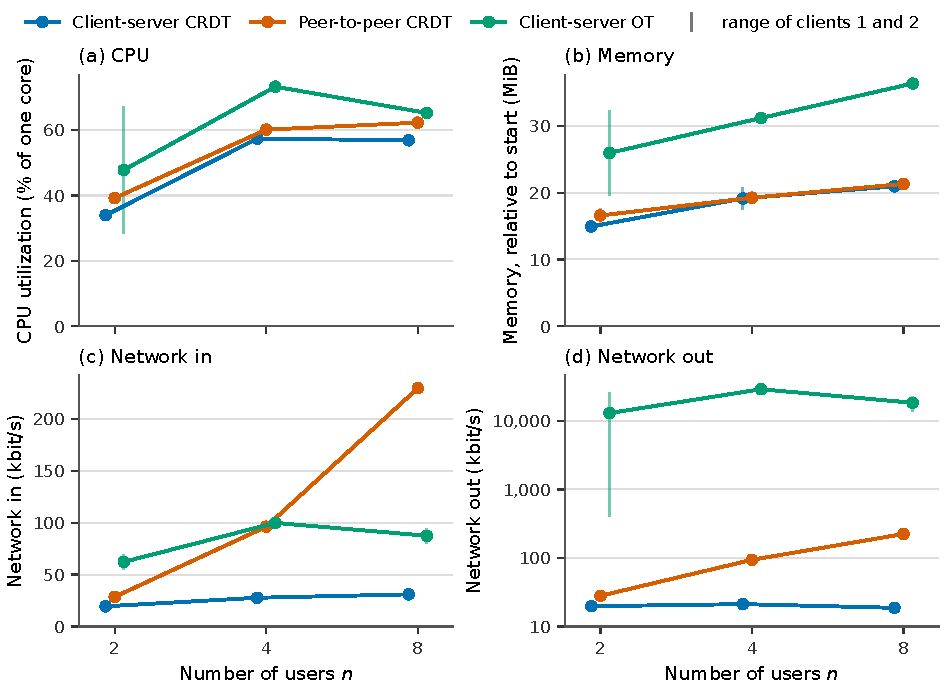
\includegraphics[width=\linewidth]{figures/summary-s1-clients}
 \caption[Mean resource usage of the client application in Scenario 1 against the number of users $n$]{Mean resource usage of the client application in Scenario 1 against the number of users $n$ (Table~\ref{tab:resource-client-1}). Each point is the mean of the first two clients; the thin bars span the two clients' own values. Network out is on a logarithmic scale.}
 \label{fig:5:summary-clients}
\end{figure}

Overall, the client-server CRDT variant is the lightest on the clients. In terms of CPU, on test machines with two vCPU cores (a maximum utilization of 200\%), every variant in Scenario 1 with $n \geq 4$ uses on average only about a third of the CPU, as Figure~\ref{fig:2-19} shows. These numbers should be read with the caveat that Scenario 1 is a much heavier load than normal use is expected to be. The operating system also decides which processes to prioritize, in memory and in CPU, while the application runs, so resource usage may be higher or lower depending on other activity on the machine.

\begin{figure}[htbp]
 \centering
 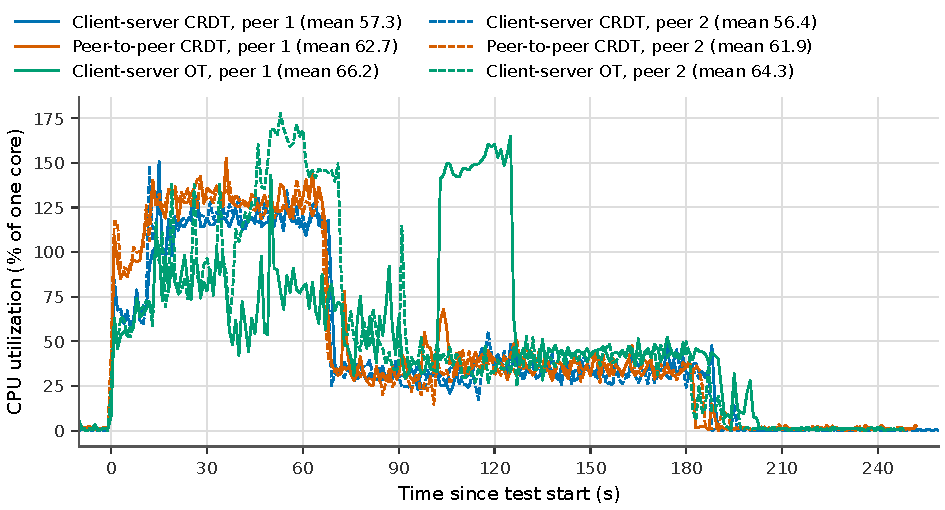
\includegraphics[width=\linewidth]{figures/s1-n8-peers-cpu}
 \caption{CPU utilization of the first and second clients, Scenario 1, $n = 8$.}
 \label{fig:2-19}
\end{figure}

\begin{figure}[htbp]
 \centering
 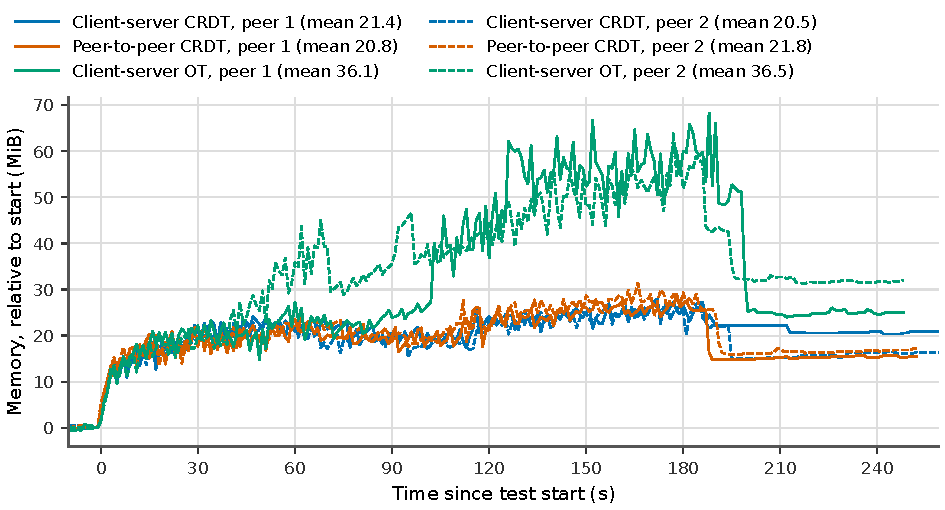
\includegraphics[width=\linewidth]{figures/s1-n8-peers-memory}
 \caption{Memory growth of the first and second clients, Scenario 1, $n = 8$.}
 \label{fig:2-21}
\end{figure}

Before normalization, memory usage starts at about 200~MiB on average, and then grows as Figure~\ref{fig:2-21} shows. Both CRDT variants grow less than the OT variant. Every variant, however, uses little memory compared with the capacity of the test machine, about 15\%. As long as the application does not load the machine to the point of disrupting the user's work, every variant of PeerToCP meets the lightweight aspect in terms of CPU and RAM.

\begin{table}[htbp]
 \centering
 \caption[Mean resource usage of the servers in Scenario 1]{Mean resource usage of the servers in Scenario 1, in the same units as Table~\ref{tab:resource-client-1}. For the peer-to-peer variant, the server is the signaling server.}
 \label{tab:resource-server-1}
 \begin{tabular}{@{}llrrr@{}}
 \toprule
 \textbf{Variant} & \textbf{Metric} & $n = 2$ & $n = 4$ & $n = 8$ \\
 \midrule
 Peer-to-peer CRDT & CPU     & 0.01     & 0.02     & 0.10 \\
                   & RAM     & 0.67     & $-$0.03  & 0.40 \\
                   & Net in  & 10.72    & 14.81    & 60.72 \\
                   & Net out & 10.24 & 15.79 & 83.11 \\
 \midrule
 Client-server CRDT & CPU     & 0.93     & 1.29      & 1.68 \\
                    & RAM     & 5.01     & 6.83      & 9.54 \\
                    & Net in  & 73.26    & 176.64    & 324.19 \\
                    & Net out & 71.79 & 193.90 & 391.66 \\
 \midrule
 Client-server OT & CPU     & 4.85        & 14.18       & 24.33 \\
                  & RAM     & 30.92       & 41.88       & 69.99 \\
                  & Net in  & 52{,}318.08    & 167{,}768.04   & 308{,}540.87 \\
                  & Net out & 26{,}494.76 & 84{,}932.31 & 156{,}178.28 \\
 \bottomrule
 \end{tabular}
\end{table}

Resource usage on the server is the other half of the lightweight aspect (Table~\ref{tab:resource-server-1}). The WebRTC signaling server of the peer-to-peer CRDT variant used minimal RAM and CPU. In the client-server architectures the server does much more: besides maintaining the connections of the clients in a network group, it keeps their replicas consistent. The server of the client-server CRDT variant sends and receives 1.4 to 2.6 times as much data as a single peer in the peer-to-peer variant.

\begin{figure}[htbp]
 \centering
 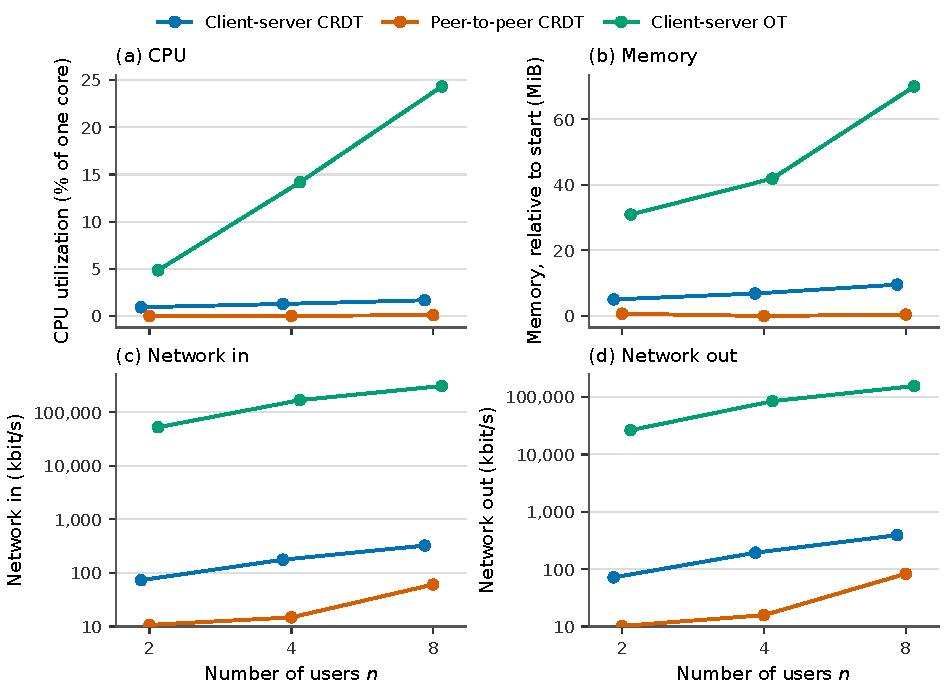
\includegraphics[width=\linewidth]{figures/summary-s1-server}
 \caption[Mean resource usage of the servers in Scenario 1 against the number of users $n$]{Mean resource usage of the servers in Scenario 1 against the number of users $n$ (Table~\ref{tab:resource-server-1}). For the peer-to-peer variant, the server is the signaling server. Network in and out are on logarithmic scales.}
 \label{fig:5:summary-server}
\end{figure}

\begin{figure}[htbp]
 \centering
 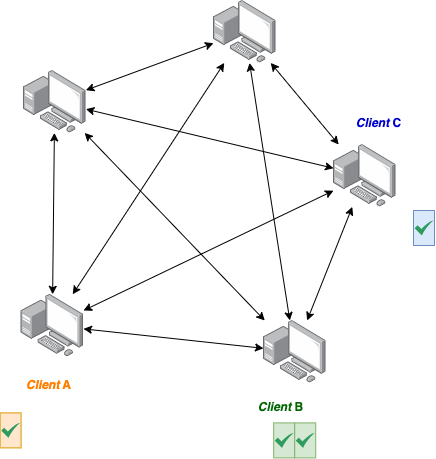
\includegraphics[width=4.08cm]{figures/crdt-sync-1}\hfill
 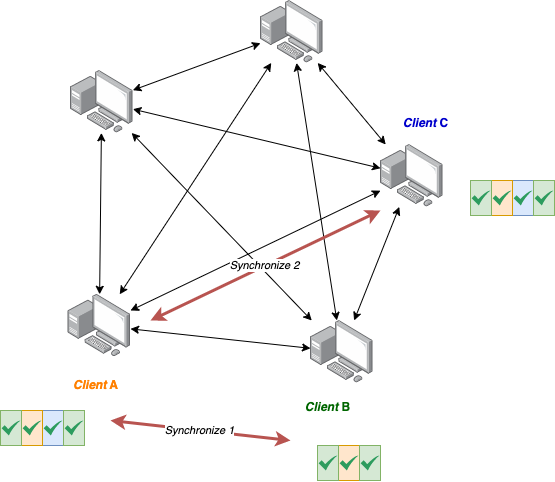
\includegraphics[width=4.8cm]{figures/crdt-sync-2}\hfill
 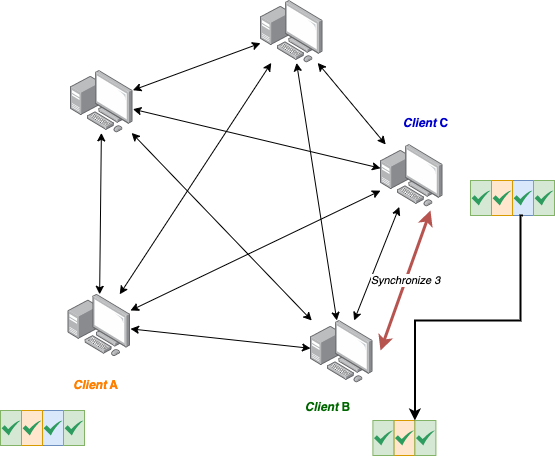
\includegraphics[width=4.8cm]{figures/crdt-sync-3}
 \caption[Synchronization in the peer-to-peer CRDT variant]{Synchronization in the peer-to-peer CRDT variant. Client A synchronizes with client B, then with client C; when B and C then synchronize, C only sends what B has not already received from A.}
 \label{fig:syncCRDT}
\end{figure}

The Yjs CRDT keeps a logical timestamp in the form of a state vector, which records the version of every user in the network. When two users synchronize, only the difference between their versions, derived from their state vectors, is sent; if the documents differ too much, the whole document may be sent instead, which can be smaller. Changes derived from the state vector are commutative and idempotent: the same change can be applied repeatedly and in any order without affecting the convergence of the document. Because of these properties, the data sent to each client does not depend on the number of operations performed, but on the size of the changes at the time of synchronization.

In Figure~\ref{fig:syncCRDT}, if client A first synchronizes with client B, then client A synchronizes with client C, and then client B synchronizes with client C, client C only needs to send B what B has not already received from client A. And if an object in the data structure is deleted before it has been synchronized, its content never needs to be sent at all. These are among the Yjs optimizations that reduce the total bandwidth between users in the CRDT variants.

Some reference implementations add an external database to store documents in the client-server architecture, so that a network group can hold more documents. None of the variants here uses a third-party database; each keeps only simple built-in data structures on the server. In the peer-to-peer architecture, documents can instead be persisted in the local storage of each peer.

\begin{figure}[htbp]
 \centering
 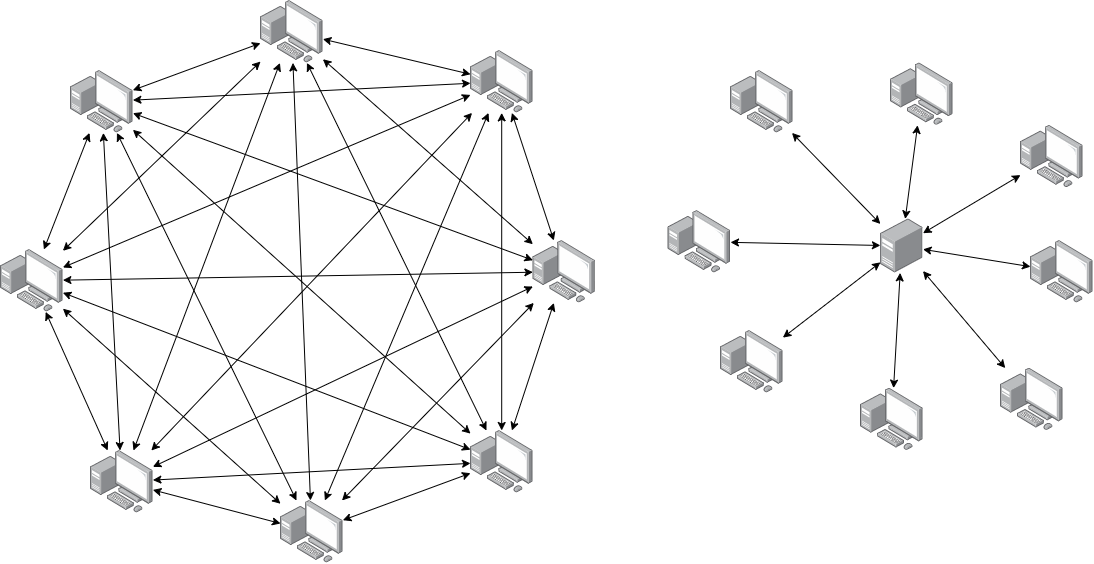
\includegraphics[width=11cm]{figures/mesh-vs-star}
 \caption{Connections in a peer-to-peer full mesh (left) and in a client-server star (right), for eight users.}
 \label{fig:compare}
\end{figure}

The price of the client-server CRDT variant's light traffic on the clients is heavier traffic on the server. In the peer-to-peer variant, on the other hand, the number of data channel connections grows quadratically with the number of users (Figure~\ref{fig:compare}), so the total traffic each peer must handle grows faster with the size of the network group. The OT variant, given its conflict-resolution protocol, has by far the largest network load of all the variants, which also drives up its CPU and RAM usage. From the lightweight perspective, the client-server OT variant is not preferred, and its data transmission protocol needs to be revisited and optimized. More sophisticated and better-optimized OT algorithms also deserve further study, so that intensive editing such as in Scenario 1 can be handled.

\chapter{Conclusion}
\label{bab:6}

This chapter concludes the study. It summarizes how each variant of PeerToCP was implemented and what the evaluation implies, and it outlines further development and experiments that could address the weaknesses found and lead to better systems of this kind.

\section{Conclusions}
\label{sec:kesimpulan}

This study set out to build PeerToCP, a real-time collaborative code editor with a shared shell. The application keeps data consistent in a distributed system with several architectures and algorithms: the operational transformation (OT) algorithm on a client-server architecture, the conflict-free replicated data type (CRDT) data structure on a client-server architecture, and a CRDT on a WebRTC-based peer-to-peer architecture.

The OT variant of PeerToCP relies on transformation property~1 (TP1) to keep every user's data in a network consistent. Every change is represented as an update operation, and both clients and server store the sequence of these operations. A client synchronizes its document with the other clients in the network by pulling updates from the server. A client may push updates to the server only if it already has the server's latest version. Otherwise, the client receives the server's newest operations and applies operational transformation to all of its local operations that the server has not yet accepted. The shared shell follows the same approach as the code editor, but its operational transformation is taken to run in constant time, because every operation is an append to an array.

Besides OT, there is the CRDT variant, which is essentially a further development of the OT algorithm with an additional data structure. PeerToCP uses the Yjs library, which implements the YATA CRDT. Every character in this data structure has its own ID. YATA stores the characters as a linear sequence, in which the position of a character is represented by its relation to the characters before and after it. This data structure is connected to a client-server network provider through the WebSocket-based y-websocket library. The peer-to-peer CRDT variant instead uses the WebRTC-based y-webrtc library, which uses WebSocket to talk to its signaling server. Both network providers give Yjs an abstraction for communicating with the other users in the network and synchronizing documents.

Every variant of PeerToCP has been shown correct theoretically, by the developers of the code it builds on, and empirically, through the four scenarios of this study. The main variant, the peer-to-peer CRDT, achieved the best latency and lower resource usage in the user's application. The OT variant suffered from excessive network bandwidth, because of a suboptimal protocol and poor concurrency of updates. This happens when every client in a network group keeps pushing updates at the same time. The server then tends to reject the update of a client whose local operations have piled up, because it gives priority to the version increments of other clients that push smaller updates.

Each variant also has its own strengths and weaknesses in how lightweight it is, on the server and in the user's application. Based on the test scenarios of this experiment, for groups of $n \leq 8$ users located close to one another, PeerToCP with the WebRTC-based peer-to-peer CRDT is the best choice. Its server load is also much lower than in the client-server architectures: in the peer-to-peer variant every computation happens on the users' own machines, so the signaling server only handles users connecting to and disconnecting from a network.

For larger network groups, the client-server CRDT variant is worth considering, because its data transmission grows more slowly with the number of clients. It is also an option when some users in the network cannot keep a WebRTC connection, because they are far apart, or because a network mechanism prevents them from connecting directly to other peers.

\section{Future Work}
\label{sec:saran}

The results suggest developing the system further into an adaptive network that changes with its conditions. This could make the service more reliable for all its users. On the algorithm side, other, more efficient variants of operational transformation or CRDTs could replace the ones PeerToCP uses now, to lower latency and the resources the application needs. One promising optimization of the CRDT variants is to modify the CRDT map (dictionary) that stores the shell replicas: it should exploit the fact that data is only ever appended to the end of an array, with no deletions or changes at any other index.

Beyond algorithms, networking and web technologies also deserve attention. HTTP/3, the newest version of HTTP at the time of this study, provides WebTransport, which could be studied as a replacement for WebSocket. WebTransport aims to offer a better programming interface, with all the features of WebSocket and a lower latency. Scalability to larger numbers of users could be tested by changing the test harness so that it no longer drives the user interface end to end. The front end and the human-computer interaction (HCI) aspects of PeerToCP could also be improved and studied.

The application could also be extended to a web version that runs without a desktop framework such as Electron, with the drawback that a web client cannot host a shell for every user in the network to share. Other technologies and programming languages with better performance and lighter resource usage than Node.js and Chromium in Electron could replace the current framework; Tauri and Qt are among the alternatives considered for PeerToCP.


\begingroup
\setstretch{1.0}
\renewcommand{\bibname}{References}
\clearpage
\phantomsection
\addcontentsline{toc}{chapter}{References}
\markboth{References}{}
\bibliographystyle{apacite}
\bibliography{references}
\endgroup

\appendix
\chapter{Code and Experimental Setup}
\label{appendix:implementation}

All code, the client application and the test experiments of this study are available at \url{https://github.com/hockyy/peertocp}. Each variant of PeerToCP is a separate branch: \texttt{crdt-cs}, the client-server CRDT variant; \texttt{ot-cs}, the client-server operational transformation variant; and \texttt{crdt-p2p}, the peer-to-peer CRDT variant. Instructions for rerunning the tests and their scenarios are in the README.md of the \texttt{crdt-p2p} branch, the repository's default branch. The servers and the modified connection providers used by each branch are available at:

\begin{itemize}
    \item \texttt{crdt-cs}: \url{https://github.com/hockyy/y-websocket};
    \item \texttt{crdt-p2p}: \url{https://github.com/hockyy/y-webrtc};
    \item \texttt{ot-cs}: \url{https://github.com/hockyy/peertocp-ot-server}.
\end{itemize}

For the experiments, every instance was set up with the following commands.

\begin{lstlisting}[language=bash]
sudo apt install -y git wget screen nginx python-is-python3 g++ make
sudo apt install -y build-essential clang libdbus-1-dev libgtk2.0-dev \
                       libnotify-dev libgnome-keyring-dev libgconf2-dev \
                       libasound2-dev libcap-dev libcups2-dev libxtst-dev \
                       libxss1 libnss3-dev gcc-multilib g++-multilib libasound2 xvfb
export DISPLAY=192.168.0.5:0.0
curl https://my-netdata.io/kickstart.sh > /tmp/netdata-kickstart.sh && sh /tmp/netdata-kickstart.sh
curl -o- https://raw.githubusercontent.com/nvm-sh/nvm/v0.39.2/install.sh | bash
source ~/.bashrc
nvm install 16
nvm use 16
git clone [URL]

# Use xvfb, because Debian has no desktop
xvfb-run npm start
\end{lstlisting}

The measurements were downloaded and processed on a local machine with the following script, which fetches the evaluation logs.

\begin{lstlisting}[language=bash]
netd () {
    curl "http://$1:19999/api/v1/data?chart=apps.mem&dimension=node \
          &after=$2&points=0&group=average&gtime=0 \
          &timeout=0&format=csv&options=seconds" \
          > mem-$3.csv
    curl "http://$1:19999/api/v1/data?chart=system.ip \
          &after=$2&points=0&group=average&gtime=0 \
          &timeout=0&format=csv&options=seconds" \
          > network-$3.csv
    curl "http://$1:19999/api/v1/data?chart=apps.cpu&dimension=node \
          &after=$2&points=0&group=average&gtime=0 \
          &timeout=0&format=csv&options=seconds" \
          > cpu-$3.csv
}

scpd () {
    scp -r hocky@$1:~/peertocpnext/out/ ./$2
}
\end{lstlisting}

Every server ran NGINX with the following configuration.

\begin{lstlisting}
location / {
    # First attempt to serve request as file, then
    # as directory, then fall back to displaying a 404.
    # try_files $uri $uri/ =404;
    proxy_pass http://127.0.0.1:3000;

    proxy_http_version  1.1;
    proxy_set_header Upgrade $http_upgrade;
    proxy_set_header Connection "upgrade";
    proxy_set_header Host $http_host;
    proxy_set_header X-Real-IP $remote_addr;
}
\end{lstlisting}

The raw measurements, and the notebook that visualizes and interprets them, are available at \url{https://github.com/hockyy/peertocp-benchmark}.


\end{document}
